\chapter{Prevalence modelling and regression methods}

\textcite[p. 311]{fisher1922mathematical} stated that the objective of
statistics is to reduce the data since its volume is impossible 
to comprehend by the researchers. In that sense, few parameters should represent the whole phenomenon catching the most relevant information. 
Years later, Newman studied the theory of modelling which can be divided 
in three aspects \cite[p. 161]{lehmann2012model}: 

\begin{alineas}
  \item models of complex phenomena are created by putting together 
  simple building elements that the researcher is familiar with and can 
  handle; 
  \item there are two types of models: the \textit{explanatory models}, 
  which will be focused on this work, and the \textit{interpolatory formulae}. 
  \item An explanatory theory necessitates a thorough understanding of the scientific context of the problem. In this regard, we investigated questions involving Respondent-driven sampling and prevalence estimation as introduced in Chapter \ref{ch:theoretical-background}. 
\end{alineas}

In this chapter, we develop models that enclose these ideas building each 
block separately. For a Bayesian modelling, we assume that each parameter
of the model has a probability distribution that incorporates the 
researcher's uncertainty about it. For each individual, we observe $k$ 
covariates that are possible risk factors represented by the vector 
$\x_i \in \R^{k}$ of the $i^{th}$ individual. We denote $\theta_i$ the 
probability of the $i$-th individual have been exposed to the disease
that depends on the prevalence $\theta$ and $\x_i$. We also consider the
dependence of sampling from RDS as a spatial random effect. The probability of
positive test in the $i^{th}$ individual is denoted by $p_i$.  

Another important feature of the model is that sensitivity and 
specificity have the same distribution for all individuals and 
it only depends on the test used to diagnose. This is an assumption 
that must be analysed for each particular case. For instance, COVID-19 
Sofia test has different sensitivity and specificity for symptomatic and 
asymptomatic individuals \cite[Table 1][p. 3]{mitchell2021performance}.  

From above, we develop three different models: the first considers perfect 
tests, that is, $\gamma_s = \gamma_e = 1$ and no spatial random effect; 
the second considers imperfect tests, regarding $\gamma_s$ and $\gamma_e$, 
but ignoring the RDS structure; and the third one has imperfect tests and 
RDS structure. \improve{Some considerations are made to improve the model's
limitations.}

The implementation of the following models were in the statistical computation
platform Stan \cite{carpenter2017stan} within Python Interface PyStan
\cite{pystan} which uses an implementation for HMC algorithm. All the codes
are written in \autoref{appendix:stan-codes}. For plotting the diagnosis and 
the distributions, ArviZ \cite{arviz_2019} and Matplotlib \cite{Hunter_2007}
Python packages were used. 

\section{Perfect tests}

The first model supposes the samples are independent and the test is perfect,
which means that $\theta_i = p_i$ for all $i$. Therefore it only considers the risk factors $\x_i$. 

\begin{equation}
  \label{model:perfect-tests}
  \begin{aligned}
    Y_i \mid \theta_i &\sim \bern(\theta_i), \\
    g(\theta_i) &= g(\theta) + \x_i^T\beta, 
  \end{aligned}  
\end{equation}
where $g(\cdot)$ is the $\logit$ function.
The parameter $\beta \in \R^{k}$ is the risk effects. For Bayesian inference, priors on
$\beta$ and $\theta$ must be included. We use $\beta ~ \sim \N(\mu_{\beta}, \Sigma_{\beta})$
and $\theta \sim \betadist(a^{p}, b^p)$, where the vector $\mu_{\beta}
\in \R^{k}$, the symmetric positive-definite matrix $\Sigma_{\beta} \in
\R^{k\times k}$, and the positive real values $a^p, b^p \in \R_{>0}$ are fixed
hyperparameters. Inferences about $\beta$ and $\theta$ are based on the
posterior distribution. Keeping the notation of
Section \ref{sec:glm}, we denote $\boldsymbol{X}$ the covariate matrix. 

\begin{remark}[Interpretation of prevalence]
  \label{remark:interpretation-prevalence}
  According to the model formulation, if the risk factors are zero, i.e $\x_i
  = 0$, the probability of the $i$-th individual having been exposed is the prevalence $\theta$, which means that in
a population with no risk effects, the probability of a person having the
disease is exactly the proportion in this population. 
\end{remark}

\subsection{Identifiability}
\label{sec:perfect-test-identifiability}

A formal definition for identifiability regards the likelihood function \cite[p.
3459]{xie2006measures}:

\begin{definition}
  \label{def:identifiability}
  Let $\mathcal{P} = \{P_{\theta} : \theta \in \Theta\}$ be
  the family of probability distributions for $\mathcal{Y}$. This model is
  {\em identifiable} if for any $\theta', \theta'' \in
  \Theta$, 
  $$\forall y \in \mathcal{Y}, P_{\theta'}(Y = y) =
  P_{\theta''}(Y = y) \implies
  \theta' = \theta''.$$ 
\end{definition} 

The family distribution from model \eqref{model:perfect-tests} is the logistic
regression parametrized by $(\theta, \beta)$ and conditioned on
observing the regressor $\boldsymbol{X}$, with $\mathcal{Y} = \{0,1\}^n$. Defining $\beta_0 =
g(\theta)$, we may rewrite it as 
$$Y_i \mid \tilde{\beta}, \tilde{\x}_i \sim \bern(g^{-1}(\tilde{\x}_i^T\tilde{\beta})),$$
such that $\tilde{\beta}$ concatenate $\beta_0$ and $\beta$, and $\tilde{\x}_i$
concatenate $1$ and $\x_i$. \textcite[p. 7]{kuchenhoff1995identification}
gives a formal proof for the identifiability of this representation.

In the Bayesian paradigm, inferences are based on the posterior distribution.
Therefore, identifiability should consider the prior distribution.
\textcite[p. 46]{lindley1972bayesian}  argued that proper priors are
sufficient to handle
identifiability problems in the Bayesian perspective, which means that a
well-defined posterior probability distribution is enough for parameter
identification. A formal definition for {\em Bayesian identifiability} is the
following: if $p(\theta \mid \beta, y, \boldsymbol{X}) = p(\theta \mid
\beta)$, the data $y$ is uninformative for $\theta$ when $\beta$ is known. 
The definition is analogous if $\beta$ and $\theta$ change places. However,
\textcite[p. 248]{gelfand1999identifiability} proved that this definition is equivalent to
likelihood identifiability. 

Despite the identifiability of the model, it may be hard to sample from
the posterior distribution depending on the value of $\x$. As an example, 
consider the following experiment: 

\begin{enumerate}[label=(\roman*)]
  \item generate $500$ covariates $X_i \sim \N(15, 1)$;
  \item let $\beta = 0.1$, $\theta = 0.1$, and $\theta_i = g^{-1}(g(\theta) +
  X_i\beta)$ for $1 \le i \le 500$;
  \item for each $i$, sample $Y_i \sim \bern(\theta_i)$;
  \item let $a^p = 1$, $b^p = 1$, $\mu_{\beta} = 0$, and $\Sigma_{\beta} = 1$
  the hyperparameters for the prior distributions (weakly informative);
  \item make 1000 warm-up and 1000 sampling iterations using Stan given the
  data $(Y_1, X_1), \dots, (Y_n, X_n)$.  
  \item make 2000 warm-up and 2000 sampling iterations using Stan given the
  data $(Y_1, X_1), \dots, (Y_n, X_n)$.
\end{enumerate}

The HMC sampler took around 8.39s.
\autoref{fig:result-uncentered-mean} presents the results through the posterior
distribution, the trace plot, and the strong posterior
correlation between $\theta$ and $\beta$. To address this 
problem, subtracting the mean $\bar{x}$ is a default procedure \cite[p.
5]{ogle2020ensuring}. After centering the data around the mean, the HMC
sampler took around 1.39s, and the improved results are shown in
\autoref{fig:result-centred-mean}. 

\begin{figure}
  \centering  
  \caption{\label{fig:result-uncentered-mean}Posterior
  distribution, trace plot, and posterior samples of parameters 
  $\theta$ and $\beta$ from model \eqref{model:perfect-tests} with uncentered covariate.}
  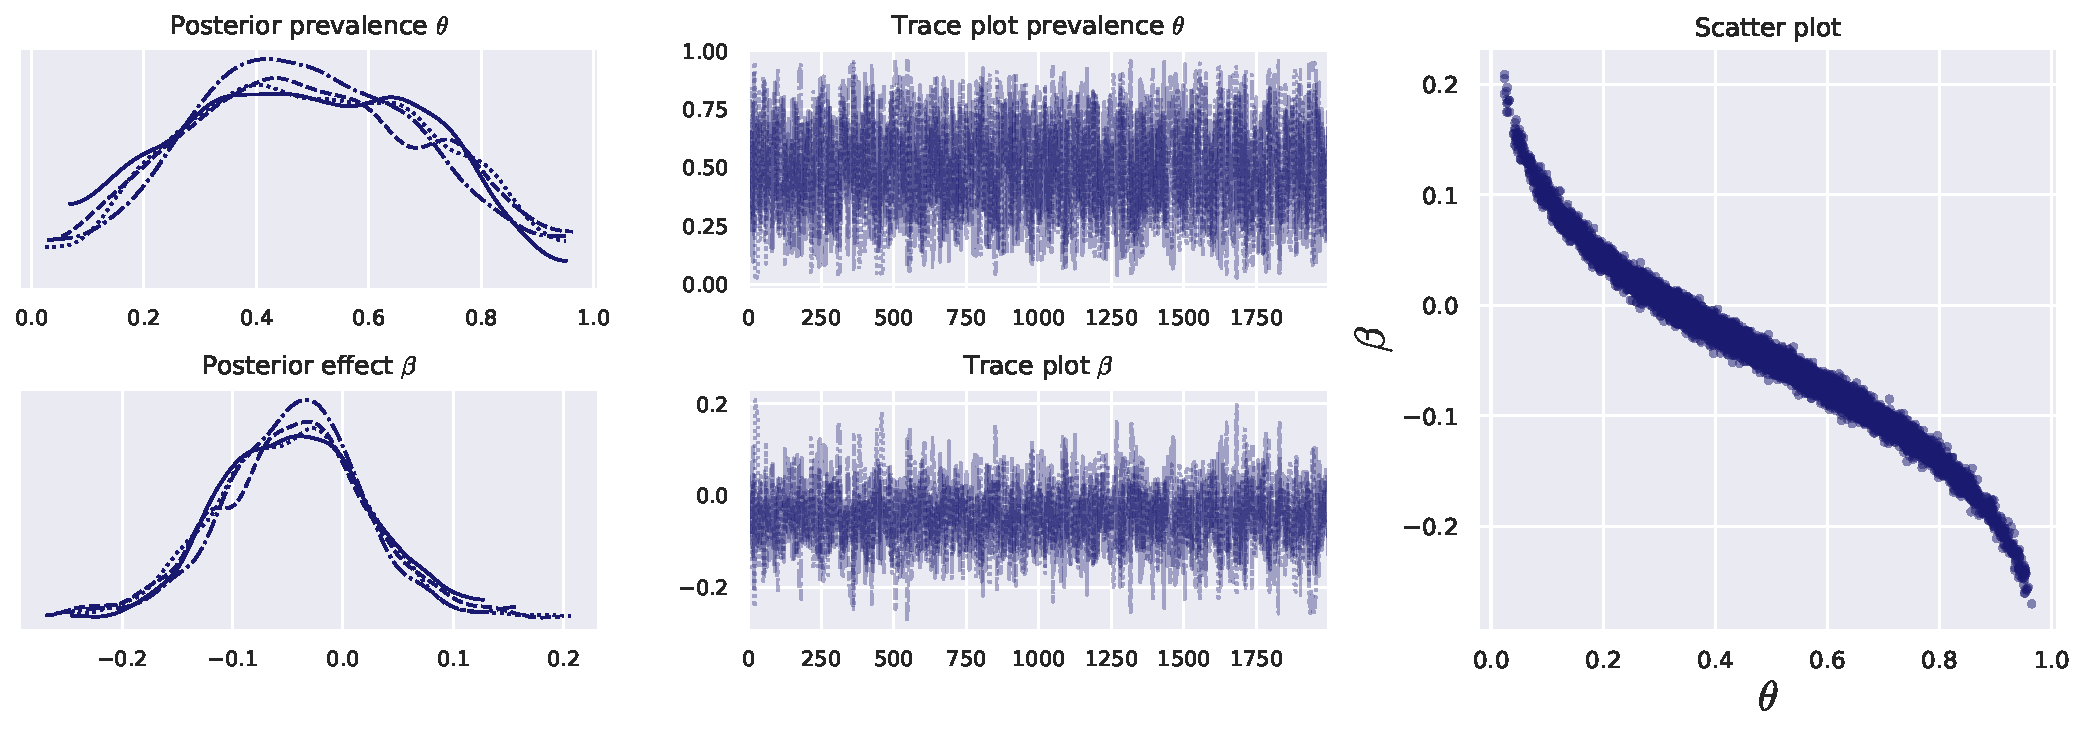
\includegraphics[width=14cm]{identifiability_perfect_tests_unscaled_x.pdf}
  \fonte{Prepared by the author (2021).}
\end{figure} 

\begin{figure}
  \centering  
  \caption{\label{fig:result-centred-mean}Posterior
  distribution, trace plot, and posterior samples of parameters 
  $\theta$ and $\beta$ from model \eqref{model:perfect-tests} with centralized covariate.}
  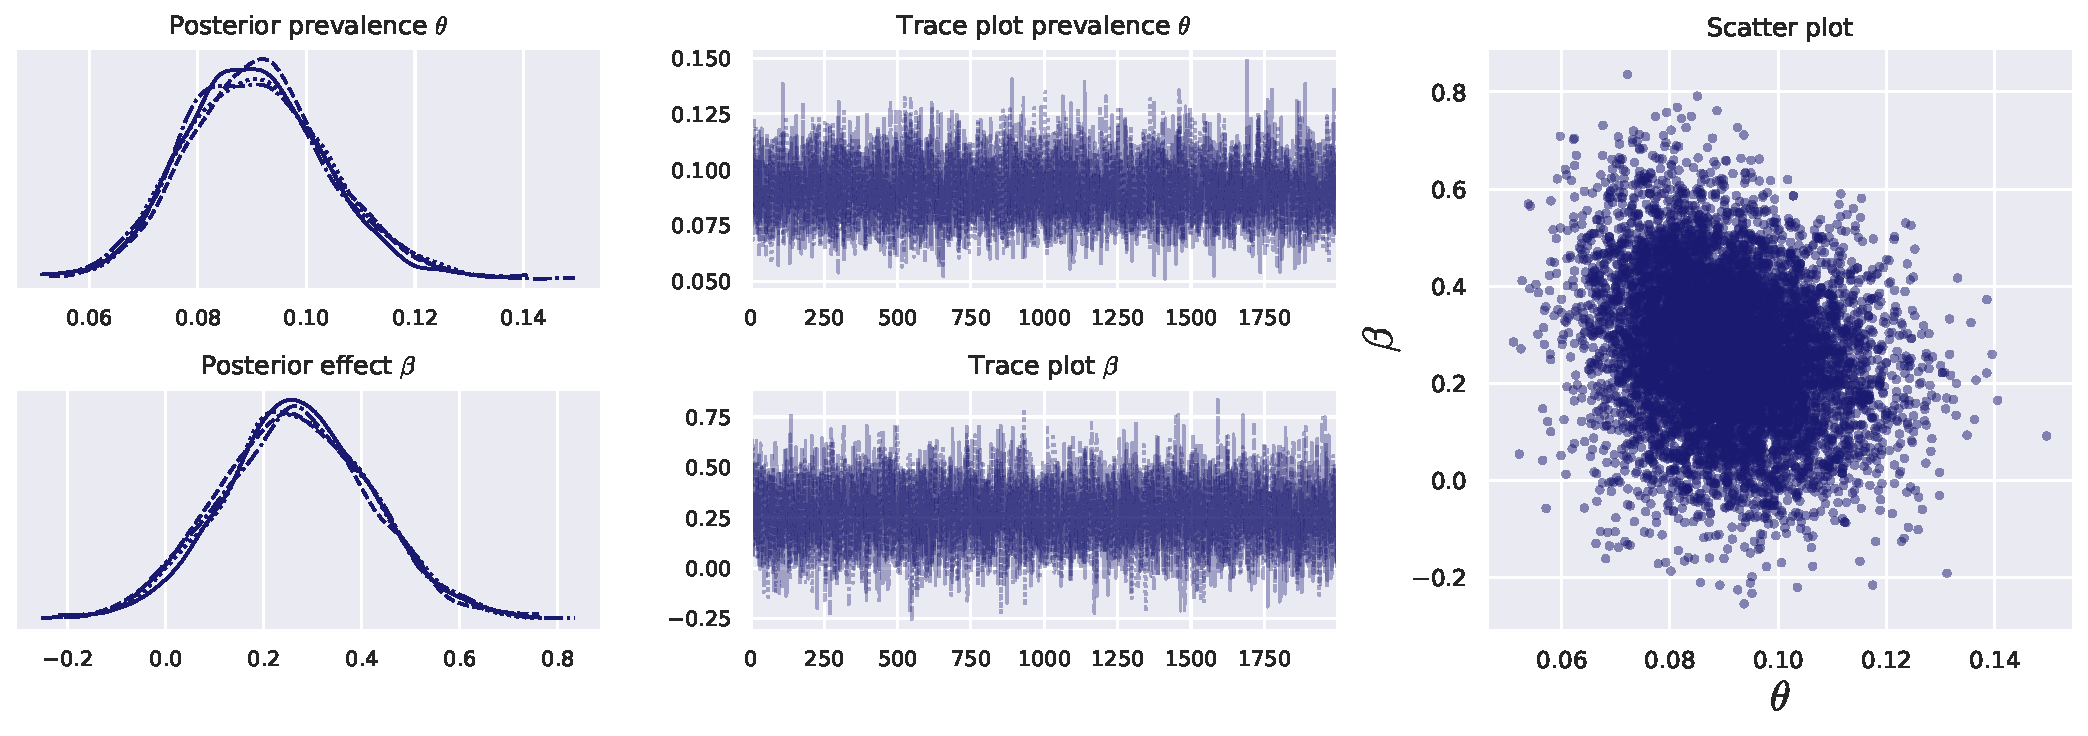
\includegraphics[width=14cm]{identifiability_scaled_x.pdf}
  \fonte{Prepared by the author (2021).}
\end{figure} 

We observe that the interpretation of prevalence from Remark
\ref{remark:interpretation-prevalence} changes from centred and 
uncentered since the meaning of $\x_i = 0$ is different. Along with this
discussion, it is usual to divide the centred variable by its
standard deviation, to put all predictors on a common scale. Discussions about
the problems caused by standardizing are outside the scope of this work. 
\textcite{gelman2008scaling} suggests to divide de continuous variables by 2
times de standard deviation to allow ``the coefficients to be interpreted in
the same way as binary deviation.'' \cite[p. 2867]{gelman2008scaling} Binary
inputs are not standardized since their coefficients are easily interpretable.

Other identifiability problems arising from the input variables are
collinearity and {\em separation} \cite[p. 1360-1361]{gelman2008weakly}. 
The latter occurs if a linear combination of a subset of the predictors gives
a perfect prediction for the binary outcome. For instance, when a linear
combination of the predictors is greater than a threshold if and only if $y =
1$.  

\subsection{Simulated data}

To present a sanity check about the functionality of model
\eqref{model:perfect-tests} and to validate the properties of the estimation
procedure, we simulate fake data from the model and make inferences about the
result. We follow the experiment from Section
\ref{sec:perfect-test-identifiability}.
\autoref{table:experiments-perfect-test} summarizes the experiment
parameters. 

\begin{table}[!ht]
  \centering
  \caption{\label{table:experiments-perfect-test}Experiment settings for the
  simulation of model \eqref{model:perfect-tests}.}
  \begin{tabular}{ccccccc}
  \hline
  Exp & $n$ & $k_{c}$ (normal) & $k_{c}$ (cauchy) & $k_{b}$ & $\beta$ & $\theta$ \\ \hline
  \multicolumn{1}{c}{1} & 100 & 3 & 0 & 2 & {[}-0.1, 2.5, 1.4, -1.8, 0.3{]} & 0.05 \\
  \multicolumn{1}{c}{2} & 100 & 3 & 0 & 2 & {[}-0.1, 2.5, 1.4, -1.8, 0.3{]} & 0.9 \\
  \multicolumn{1}{c}{3} & 100 & 2 & 2 & 1 & {[}-0.1, 2.5, 1.4, -1.8, 0.3{]} & 0.1 \\
  \multicolumn{1}{c}{4} & 5000 & 40 & 5 & 5 & $F$ distribution & 0.1 \\\hline
  \end{tabular}
  \fonte{Prepared by the author (2021). We denote $n$ for number of samples,
  $k_c$ for the number of continuous variables, and $k_b$ for binary variables. Between
  paranthesis, \textit{normal} means that the variables were generated from a
  Multivariate Normal with prespecified parameters, and \textit{cauchy} from a
  Cauchy distribution. $F$ distribution is $\N(\mu = 0, \sigma = 2)$ with
  probability 0.3, and 0 otherwise.}
\end{table}

We primally look at the settings from experiment 1. With a non-informative prior for $\theta$
(Jeffreys prior $\betadist(1/2, 1/2)$) and a weakly informative for $\beta$
(zero mean and covariance matrix four times the identity matrix),
\autoref{fig:result-experiment1-perfect-test} shows the posterior
distributions for the parameters. The prevalence estimate is good despite
Jeffreys' prior. When the distance between the prior and the true value is large, the
inferences seem to be biased. However, this makes sense regarding the model. For
instance, for $\beta_2$, before observing the data, we put 0.7 mass probability
for values less than 0.1. The data decreased it to 0.125. This highlights
the importance of a well defined prior distribution. The values for Bulk ESS
was greater than 3000 for all parameters, while Tails ESS were greater that
2200 with 1000 warmup and 1000 sampling iterations, and 4 chains. For all
parameters $\hat{R} = 1$. Trace plots and scatter plots were also good and we
omit here since they do not bring new information for the discussion. 

\begin{figure}[!ht]
  \centering  
  \caption{\label{fig:result-experiment1-perfect-test}Posterior
  distribution for parameters of model \eqref{model:perfect-tests}.}
  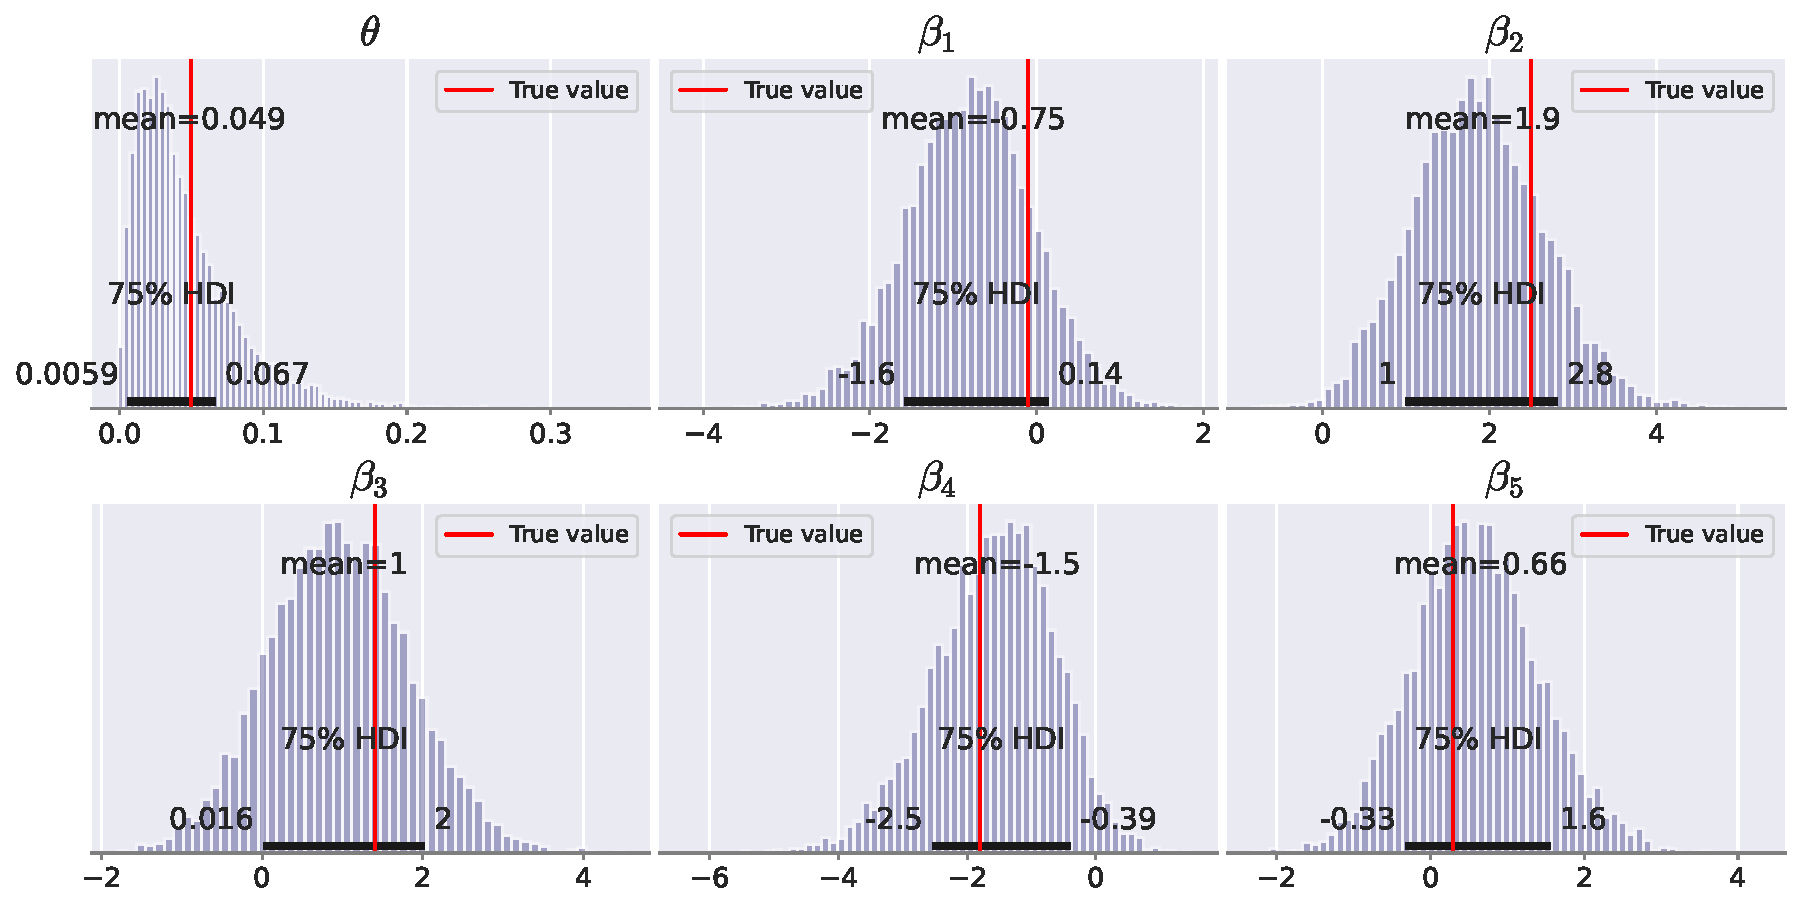
\includegraphics[width=14cm]{posterior_perfect_tests_exp1.pdf}
  \fonte{Prepared by the author (2021). The red line represents the true value
  inputed for the simulation.}
\end{figure} 

\autoref{fig:predicted-vs-simulated-perfect-tests} compares the predicted and
simulated probabilities of having the disease $\theta_i$. Although we are performing Bayesian inference, frequentist properties can be
accessed through simulation. After 1000 simulations varying the input data
$Y$, the 75\% credible interval included the true parameters in 75.8\%, 78.8\%,
76.4\%, 77.5\%, 67.3\%, and 72.2\% of the times, respectively for $\theta,
\beta_1, \dots, \beta_5$. Each simulation had 100 samples and weakly
informative priors for $\beta$ and $\theta$.

\begin{figure}[!ht]
  \centering  
  \caption{\label{fig:predicted-vs-simulated-perfect-tests}Comparing predicted
 and simulated probabilities of having the disease from model \eqref{model:perfect-tests}.}
  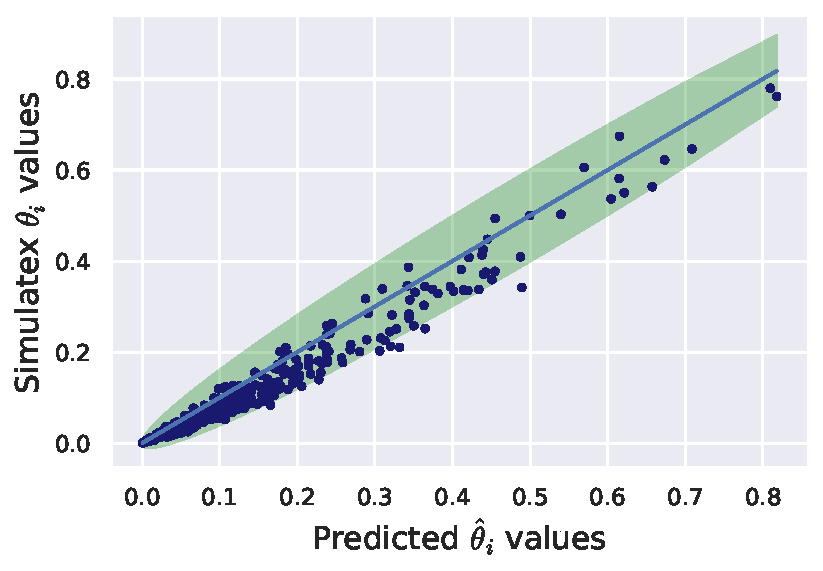
\includegraphics[width=10cm]{predicted-vs-simulated-perfect-tests.pdf}
  \fonte{Prepared by the author (2021). The green area is delimited by the curves generated
  by $2\sqrt{\theta_i(1-\theta_i)/n}$, where $n=500$ is the number of points. 
  This area is a proxy for $\pm 2$ standard-error bounds. }
\end{figure} 

Experiment 2 is used to see if these properties repeat when the prevalence is
higher. The same regressors were used for the comparison, but the input data
$Y$ were generated with different prevaleces. With prevalence being 0.9, the
estimates were a little high for all coefficients as
\autoref{fig:comparing-diff-prevalence-perfect-tests} presents. This is
related to the fact that the posterior mean underestimated the true value for this
experiment. After increasing the number of samples, the estimates were closer,
as expected. 

\begin{figure}[!ht]
  \centering  
  \caption{\label{fig:comparing-diff-prevalence-perfect-tests}Comparing
  posterior mean and 94\% credibility intervals for $\beta$ in model \eqref{model:perfect-tests} with the same regressors
  $\boldsymbol{X}$ but different prevalences.}
  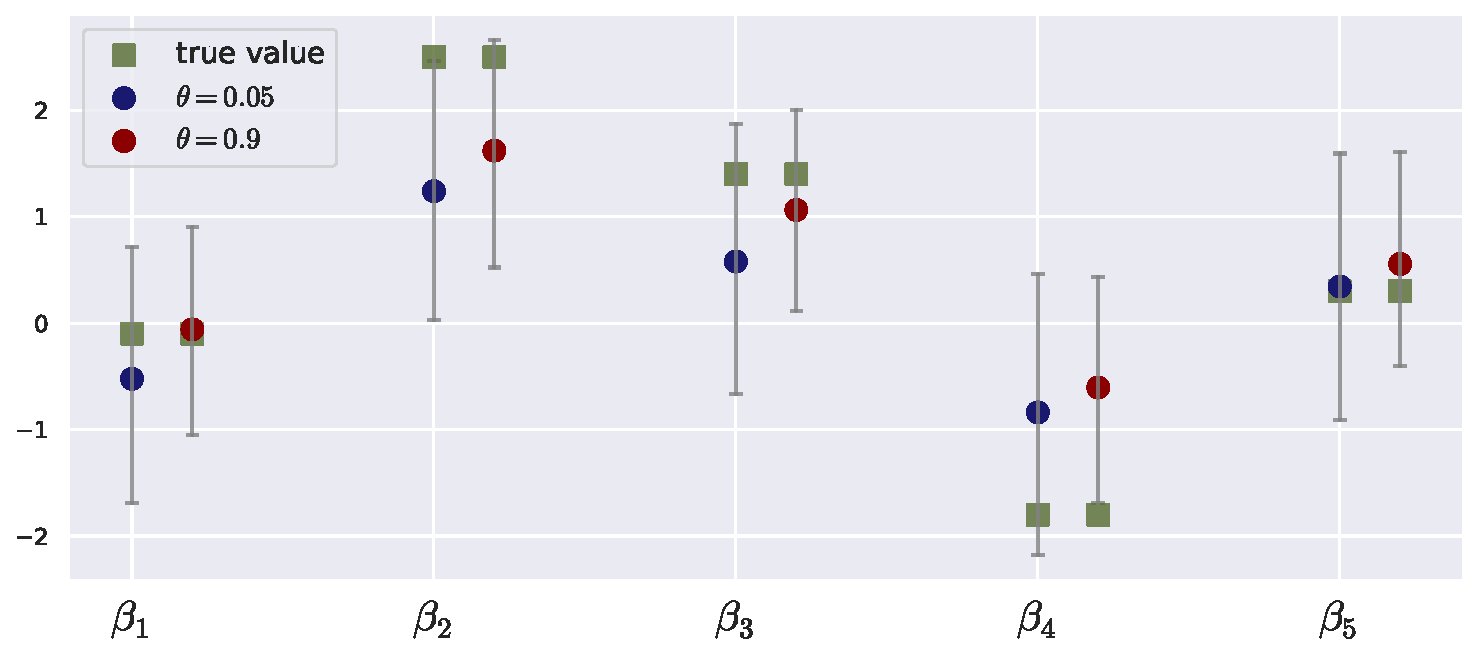
\includegraphics[width=12cm]{comparing-diff-prevalence-perfect-tests.pdf}
  \fonte{Prepared by the author (2021).}
\end{figure} 

The third experiment aims to analyse what happens if some covariates have a
heavier tail. No big difference was noticed despite the existence of some
individuals very different from the others. At last, the fourth experiment
increases the dimensionality to observe the number of effective samples. Each
chain took around 3 minutes, instead of the 3s needed for the previous
experiments. From the 51 parameters, 48 had the true values in the 95\% HDI
credible interval. The Bulk ESS was greater than 4500 for 95\% of the
parameters. \autoref{fig:predicted-vs-simulated-high-dimension-perfect-tests}
presents how the predicted probabilities for each individual behaves in this
case. 

\begin{figure}[!hb]
  \centering  
  \caption{\label{fig:predicted-vs-simulated-high-dimension-perfect-tests}
  Comparing predicted and simulated probabilities of having the disease from
  model \eqref{model:perfect-tests} with high dimension.}
  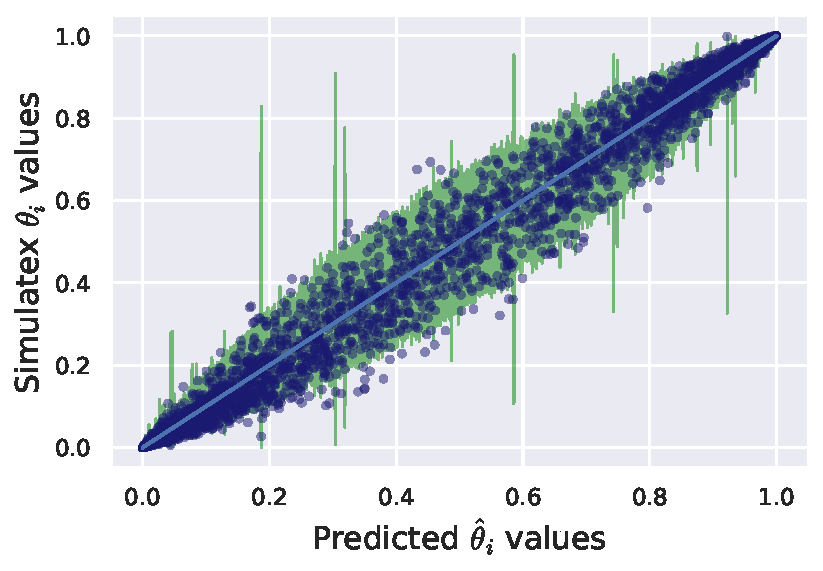
\includegraphics[width=10cm]{predicted-vs-simulated-high-dimension-perfect-tests.pdf}
  \fonte{Prepared by the author (2021). The green area indicated the 95\%
  credible interval for each predicted $\theta_i$}
\end{figure} 

\section{Sensitivity and specificity}

In this section, we describe a model for estimating the sensitivity and
specificity of a diagnostic test. This model is relevant to analyze and
experiment with different prior specification approaches. Suppose having a
gold standard test and another test, for instance, a simpler, faster, or less
invasive one, which we want to estimate the accuracy by the sensitivity and
specificity. In this scenario,
true positive (negative) individuals are those who tested positive (negative) by
the gold standard. Therefore, in a population with $n_{\gamma_s}$ true
positives and  $n_{\gamma_e}$ true negatives, we denote 
\begin{equation}
  \label{model:sensitivity-specificity}
  \begin{aligned}
    y_{\mathrm{pos}} &\mid \gamma_s \sim \operatorname{Binomial}(n_{\gamma_s}, \gamma_s),\ \\
    y_{\mathrm{neg}} &\mid \gamma_e \sim \operatorname{Binomial}(n_{\gamma_e}, \gamma_e), 
  \end{aligned}
\end{equation}
such that $y_{\mathrm{neg}}$ are negative tests on known negative 
subjects and $y_{\mathrm{pos}}$ are positive tests on
known positive. In the Two-by-two formulation from \autoref{table:two-by-two},
we have

\begin{quadro}[!ht]
  \centering
  \caption{\label{table:two-by-two-data}Two-by-two table with the model specification.}
  \begin{tabular}{c|c|c|c|}
  \cline{2-4}
                                               & $Y = 0$ & $Y = 1$ & Total\\ \hline
  \multicolumn{1}{|c|}{$Y^{\mathrm{true}}= 0$} & $y_{\mathrm{neg}}$  & $n_{\gamma_e} - y_{\mathrm{neg}}$ & $n_{\gamma_e}$ \\ \hline
  \multicolumn{1}{|c|}{$Y^{\mathrm{true}}= 1$} & $n_{\gamma_s} -
  y_{\mathrm{pos}}$    & $y_{\mathrm{pos}}$  & $n_{\gamma_s}$  \\ \hline
  \multicolumn{1}{|c|}{Total} & $n_{\gamma_s} + y_{\mathrm{neg}} -
  y_{\mathrm{pos}}$ & $n_{\gamma_e} + y_{\mathrm{pos}} - y_{\mathrm{neg}}$ &
  $n_{\gamma_s} + n_{\gamma_e}$ \\\hline
  \end{tabular}
  \fonte{Prepared by author (2021).}
\end{quadro}

In Bayesian analysis, we have to define a prior distribution with density $\pi$ for the
parameters $(\gamma_e, \gamma_s)$. For this, we consider three different approaches: 

\begin{alineas}
  \item prior distributions are specified independently for each parameter and
  each one has a beta distribution, i.e,  
  $$\pi(\gamma_e, \gamma_s) =
  \pi(\gamma_e)\pi(\gamma_s) \propto \gamma_s^{a_s}(1-
  \gamma_s)^{b_s}\gamma_e^{a_e}(1-\gamma_s)^{b_e},$$
  for $a_s, b_s, a_e,$ and $b_e$ being pre-determined positive real hyperparameters;
  \item bivariate normal distribution in the log odds space, i.e,  
  $$(\logit(\gamma_e), \logit(\gamma_s)) \sim
  \N(\mu_{\gamma}, \Sigma_{\gamma}),$$
  such that the vector $\mu_{\gamma} \in \R^2$ and the covariance matrix
  $\Sigma_{\gamma} \in \R^{2\times 2}$ are pre-determined hyperparameters;
  \item a bivariate beta distribution described in Appendix \ref{appendix:bivariate-beta-distribution}
  with parameters $\alpha_1, \dots, \alpha_4 \in \R_{>0}$.
\end{alineas}

If more studies about the same diagnostic test are available, a {\em
hierarchical partial pooling} approach can be adopted for prior specification,
as explained by \textcite[p. 1272-1274]{gelman2020bayesian} and by
\textcite[p. 2-3]{guo2017bayesian}.  

\subsection{Independent beta distribution priors}

If the knowledge of the specificity affects the range of most possible values
of the sensitivity, or vice-versa, there is antecedent information about the
correlation between the parameters. When this is not the case, a possible
independent prior formulation is the usage of $\betadist$ distribution since
it is bounded in the interval $[0,1]$ and it is reasonably flexible in its
shape.  Another good reason for this choice is that the beta distribution
forms a conjugate family with the likelihood binomial distribution (see Definition
\ref{def:conjugate-family}), which is more tractable numerically. Therefore we
have the following prior specification 
\begin{equation*}
  \begin{aligned}
    \gamma_s &\sim \betadist(a_s, b_s), \\
    \gamma_e &\sim \betadist(a_e, b_e), 
  \end{aligned}
\end{equation*}
which leads to the following posterior distribution from the likelihood
\eqref{model:sensitivity-specificity}:
\begin{equation*}
  \begin{aligned}
    \gamma_s \mid y_{\mathrm{pos}} \sim \betadist(a_s + y_{\mathrm{pos}}, b_s + n_{\gamma_s} - y_{\mathrm{pos}}), \\
    \gamma_e \mid y_{\mathrm{neg}} \sim \betadist(a_e + y_{\mathrm{neg}}, b_e + n_{\gamma_e} - y_{\mathrm{neg}}).
  \end{aligned}
\end{equation*}

Notice that this particular likelihood function does not add any correlation to the
parameters since it treats each one separately. The interpretation of the beta
distribution parameter is in terms of the number of successes for the first
parameter and failures for the second parameter. With respect to Section
\ref{sec:correlation-sensitivity-specificity}, since the likelihood from this
model does not add any correlation to the posterior distribution, the prior
distribution has to give this information to it, when necessary.  

\subsection{Bivariate normal distribution in the log odds space}

This approach was designed by \textcite{chu2006bivariate} to jointly analyse 
sensitivity and specificity from a set o studies. In their work, the prior
specification allows the incorporation of regressors. We consider it without
the regressors, which simplifies to
\begin{equation*}
  \begin{pmatrix}
    \logit(\gamma_s) \\
    \logit(\gamma_e)
  \end{pmatrix}
\sim \operatorname{Normal}(\mu_{\gamma}, \Sigma_{\gamma}), \text{ with } \Sigma_{\gamma} =  
\begin{pmatrix}
  \sigma_{\gamma_s}^2 & \rho\sigma_{\gamma_s}\sigma_{\gamma_e} \\
  \rho\sigma_{\gamma_s}\sigma_{\gamma_e} & \sigma_{\gamma_e}^2  
\end{pmatrix},
\end{equation*}
such that $\sigma_{\gamma_s} > 0$ and $\sigma_{\gamma_e} > 0$ are the
standard deviations from log odds of sensitivity and specificity,
respectively, and $\rho$ is the correlation between the parameters in the log 
odds space. The possible problem with that prior approach is that the moments
of logit normal distribution are not in closed form and there is no available
formula to derive $\ev[\gamma_s]$ from the parameters of the normal
distribution \cite{kurt2021logit}. 

\subsection{A bivariate beta prior}

A common practice is to define the beta distribution as a prior distribution
over $[0,1]$. When more dimensions are necessary, the Dirichlet distribution
is a possible generalization with the restriction that the parameters live in
the simplex of lower dimension, i.e., if $\boldsymbol{x} \in [0,1]^d$ has Dirichlet
distribution, there is the restriction $\sum_{i=1}^d \boldsymbol{x}_i = 1$.
Because of that, \textcite{olkin2015constructions} build a bivariate beta distribution
with positive probability in $(0,1)^2$, with marginals having beta
distribution and correlation over the interval $(-1,1)$. Appendix
\ref{appendix:bivariate-beta-distribution} presents a detailed derivation. The
prior specification is as follows: 
\begin{equation*}
  \begin{aligned}
    (U_1, \dots, U_4) &\sim \operatorname{Dirichlet}(\alpha_1, \dots, \alpha_4), \\
    \gamma_e &= U_1 + U_2, \\
    \gamma_s &= U_1 + U_3.
  \end{aligned}
\end{equation*}
Prior distributions can be placed on the hyperparameters $\alpha_i$. In this work,
we employ 
\begin{equation*}
  \alpha_i \sim \operatorname{Gamma}(a^i, b^i), \quad a^i, b^i > 0, \quad \text{ for } i = 1,\dots,4. 
\end{equation*}
Suppose the research have prior information about specificity and specificity,
such their mean and correlation. 

To specify the prior hyperparameters using prior information, Section
\ref{sec:elicitation-bivariate-beta} discusses the results when the
researcher prespecifies $m_s = \ev[\gamma_s], m_e = \ev[\gamma_e], v_s = \var(\gamma_s),
v_e = \var(\gamma_e)$, and $\rho  = \cor(\gamma_s, \gamma_e)$. Since system
\eqref{eq:system-moments-alpha} usually has no solution, an optimization
problem is solved with $m_s$ and $m_e$ fixed, and the other parameters being
an approximation of the researcher's input values. For more details, see Appendix \ref{appendix:bivariate-beta-distribution}.

\begin{alineas}
  \item having $\alpha_i$ fixed: we search for $\alpha_i = \hat{\alpha}_i >
  0$ thorough the values of $m_s, m_e, \rho, v_s$, and $v_e$. An optimization
  problem is searching for $\hat{\alpha}_i$ which gives moments
  $\var(\gamma_s), \var(\gamma_e)$, and $\cor(\gamma_s, \gamma_e)$ as close as
  possible to the input values, and $m_s = \ev[\gamma_s], m_e =
  \ev[\gamma_e]$. A variation of this method would include $m_s$ and $m_e$ in
  the optimization problem and it is suggested when believes about $m_s$ and
  $m_e$ are less strong. 
  \item having $\alpha_i$ as a hierarchical parameter: we first estimate
  $\hat{\boldsymbol{\alpha}}$ the same way as described above and set
  $\ev[\alpha_i] = a^i/b^i = \hat{\alpha}_i \implies a^i = b^i\hat{\alpha}_i$.
  The parameter $b_i = \hat{\alpha}_i/\var(\alpha_i)$ is a inversely
  proportional quantity to the spread of parameter $\alpha_i$. The interesting
  thing about this approach is that it allows the prior to move more freely,
  specially when the input values are far from the estimated ones. 
\end{alineas}

\subsubsection*{Implementation of the dirichlet distribution in Stan}

The Dirichlet distribution is defined on the simplex of lower dimension.
Therefore the sampler has to consider the restriction of $\sum_{i=1}^4 U_i =
1$. \textcite{betancourt2012cruising} presents a simplification in the
structure of the simplex. The propose is \cite[p. 2]{betancourt2012cruising}
\begin{equation*}
  \begin{aligned}
    z_i &\sim \betadist(\tilde{\alpha}_i, \alpha_i), \text{ where } \tilde{\alpha}_i = \sum_{k=i+1}^4 \alpha_k, \quad i = 1,2,3 \\
    U_i &= \left(\prod_{k=1}^{i-1} z_k\right)\cdot \begin{cases}
      1 - z_i, &i < 4 \\
      1, &i = 4
    \end{cases},
  \end{aligned}
\end{equation*}
which removes the constraint. 

\begin{remark}
  When $\alpha$ is a random variable, the adapt delta parameter had to be
  increased to 0.9, since some divergences were found. 
\end{remark}

\subsection{Comparing the prior specifications with simulated data}

Now we are going to compare the three prior specification methods. For each of
the following three situations, we are going to simulate 1000 datasets from
the binomial likelihood with $n_{\gamma_s}, n_{\gamma_e} \sim
\operatorname{Poisson}(50)$, $\gamma_s \sim \betadist(100, 0.15/0.85 \cdot
100)$ to ensure $\ev[\gamma_s] = 0.85$, and  $\gamma_e \sim \betadist(100, 0.2/0.8 \cdot
100)$ to ensure $\ev[\gamma_e] = 0.8$. The three situations are: 

\begin{alineas}
  \item \label{item:vague-information-sensitivity-specificity} only vague information is available; 
  \item \label{item:strong-mean-sensitivity-specificity} strong beliefs about the means and no information about correlation; 
  \item\label{item:strong-mean-cor-information-sensitivity-specificity}  strong beliefs about the means and the correlation. 
\end{alineas}

For each situation and each dataset, it was drawn 2000 samples from the
posterior distribution and the HDI 75\% interval and posterior mean were calculated. The Hits
column counts the percentage of the times that the true values lied in the
interval, while the MSE column calculates the mean squared error of the
posterior mean with respect to the true value. We notice that the fourth prior
approach had a little number of effective samples when compared to the other
methods.  Notice that there is no big different among the approaches. The
logit normal prior is worst when strong information is given. This may be
related to the difficulty to convert information from the probability space to
the log odds space. The estimation error decreased when information about the 
means and correlation is given.
\autoref{fig:comparing_hdi_prior_approaches_sens-spec} 
shows that the credible intervals change very little for each different
approach and even for each quantity of information, which tells that the data 
is driving the posterior. 

\begin{table}[tbp]
  \centering
  \caption{\label{tab:comparison-prior-approach-sensitivity-specificity}Comparing
  prior specification approaches in three different situations.}
  \begin{tabular}{cccccc}
    \hline
    \multirow{2}{*}{\textbf{Situation}} & \multirow{2}{*}{\textbf{Prior
    approach}} & \multicolumn{2}{c}{\textbf{Hits}} &
    \multicolumn{2}{c}{\textbf{MSE} $10^{-3}$} \\ \cline{3-6} 
     &  & \textbf{Sens} & \textbf{Spec} & \textbf{Sens} & \textbf{Spec} \\ \hline
    \multirow{4}{*}{\autoref{item:vague-information-sensitivity-specificity}} & Independent betas & 73.8\% & 76.1\% & 2.531 & 2.843 \\
     & Logit normal & 74.1\% & 74.5\% & 2.405 & 2.811 \\
     & Biv. beta constant $\alpha$ & 75.6\% & 75.5\% & 2.388 & 2.625 \\
     & Biv. beta random $\alpha$ & 74.9\% & 74.4\% & 2.264 & 2.546 \\\hline
    \multirow{4}{*}{\autoref{item:strong-mean-sensitivity-specificity}} & Independent betas & 74.1\% & 73.6\% & 2.009 & 2.363 \\
     & Logit normal & 69.9\% & 71.2\% & 2.300 & 2.797 \\
     & Biv. beta constant $\alpha$ & 75.2\% & 75\% & 1.952 & 2.316 \\
     & Biv. beta random $\alpha$ & 74.7\% & 74.8\% & 2.167 & 2.454 \\\hline
    \multirow{4}{*}{\autoref{item:strong-mean-cor-information-sensitivity-specificity}} & Independent betas & 74.3\% & 74.2\% & 2.007 & 2.365 \\
     & Logit normal & 68.4\% & 71.5\% & 2.303 & 2.804 \\
     & Biv. beta constant $\alpha$ & 74.3\% & 74.9\% & 1.989 & 2.364 \\
     & Biv. beta random $\alpha$ & 74.5\% & 75.5\% & 2.229 & 2.504 \\ \hline
    \end{tabular}
  \fonte{Prepared by the author (2021). Biv. means bivariate and Hits is the percentage of times that the estimated HDI 75\% included the true value.}
  \end{table}

\begin{figure}
  \centering
  \caption{\label{fig:comparing_hdi_prior_approaches_sens-spec}The average
  posterior mean estimate and average HDI 75\% intervals
  for each prior strategy and level of information for sensitivity.}
  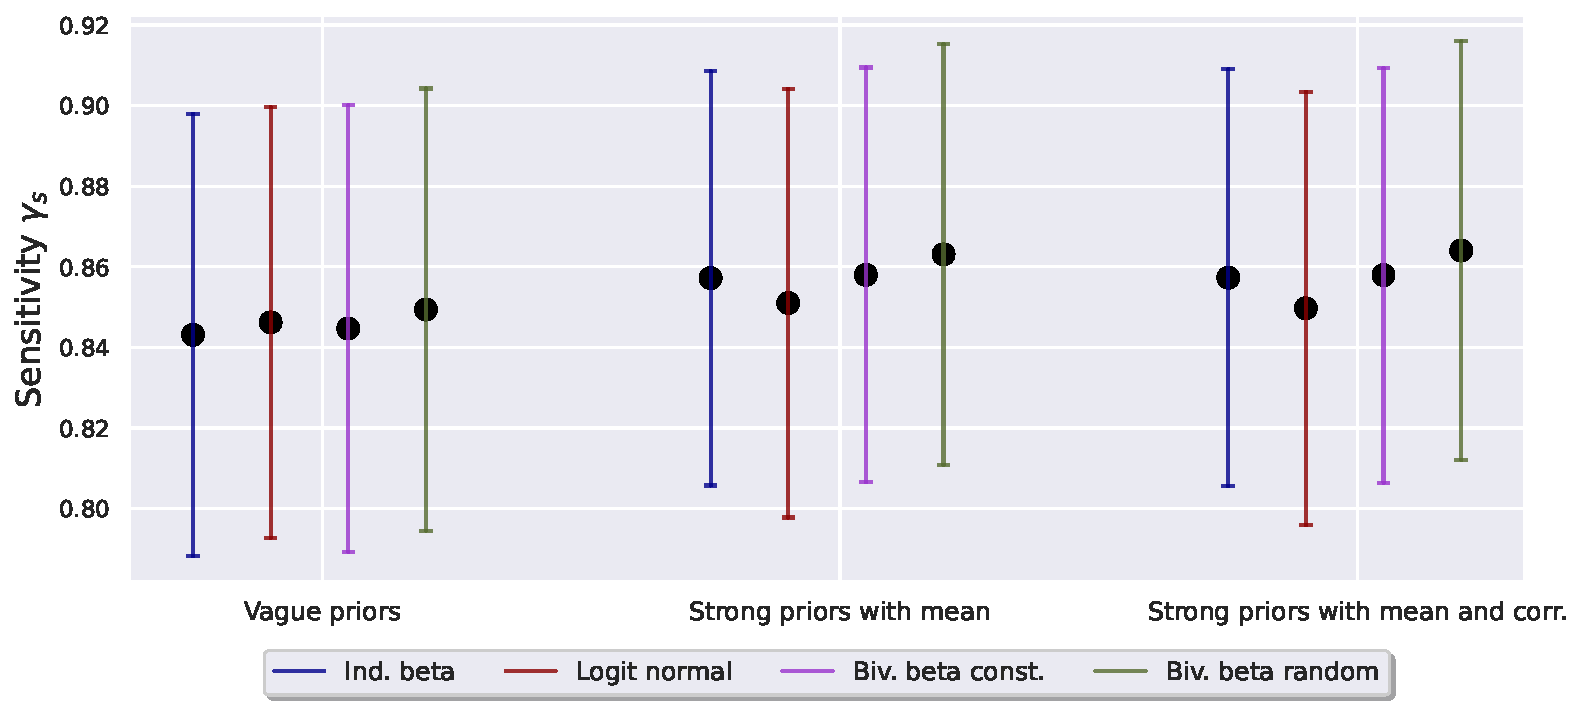
\includegraphics[width=12cm]{comparing_hdi_prior_approaches_sens-spec.pdf}
  \fonte{Prepared by the author (2021).}
\end{figure}

By the above analysis, we choose the independent betas approach given it 
reduces the computational burden. 

\section{Imperfect tests}

A slight modification of model \eqref{model:perfect-tests} is to consider 
the imperfection of the test measured through specificity and sensitivity, 
remembering the relation of these quantities to the apparent prevalence
through equation \eqref{eq:apparent-true-prevalence}. Hence, the model can be
written as
\begin{equation}
  \label{model:imperfect-tests}
  \begin{aligned}
    Y_i \mid p_i &\sim \bern(p_i) \\
    p_i &= \gamma_s\theta_i + (1-\gamma_e)(1 - \theta_i),  \\
    g(\theta_i) &= g(\theta) + \x_i^T\beta,  \\
    \beta  &\sim \N(\mu_{\beta}, \Sigma_{\beta}), \\ 
    \theta &\sim \betadist(a^p, b^p), 
  \end{aligned}  
\end{equation}
with priors on $(\gamma_e, \gamma_s)$ as studied in the previous section. It is
important to highlight that we suppose prior the data that $\theta$ is
independent of $\gamma_e$ and $\gamma_s$, which is not necessarily true as
pointed out by \textcite{leeflang2013variation}, who concluded that
specificity tends to be lower when prevalence is higher. This 
is an extension of model presented by \textcite{gelman2020bayesian} and
studied by \textcite{mcinturff2004modelling}. 

\subsection{Identifiability}

If the regressors $\boldsymbol{x}_i$ are not present in model
\eqref{model:imperfect-tests}, it is no identifiable with respect to its
likelihood as pointed out by \textcite[p. 1271]{gelman2020bayesian}. 
Intuitively, the problem happens because $Y_i$ brings information about 
$p_i$ which is subdivided in three parameters: $\theta, \gamma_s$ and
$\gamma_e$. Regarding Definition \ref{def:identifiability} and dropping the
index $i$, take $\theta = 0.1, \gamma_e = 0.9$ and $\gamma_s = 0.6$. Then, 
\begin{equation*}
    p = 1 - \gamma_e + \frac{\gamma_s + \gamma_e - 1}{1 + e^{-g(\theta)}} = 0.15.
\end{equation*}
With $\gamma_e = 0.9$, $\gamma_s = 0.2$ and $\theta = 0.5$, the value of $p$
is also $0.15$, which implies that two
different combinations of the parameters generate the same probability
function for $Y$. As a consequence, the model is non-identifiable. Including the
regressors, the calculations are harder. Suppose that $g(\theta)$
is increased by a real $a$. The effect of $a$ on $p_i$ is through
$g^{-1}(g(\theta) + a + \boldsymbol{x}_i^T\beta)$, which depends on
$\boldsymbol{x}_i$. Because of that, sensitivity and specificity can not generally
offset this difference, and identifiability can not be proved or disproved. 

Nevertheless, there are some tractable cases. For instance, if $\boldsymbol{x}_i = x_i$ is a binary variable, with the same
reasoning, it can be shown that the model is not identifiable. Moreover the
problems concerning the covariates $\boldsymbol{X}$ appear here in the same
manner. To avoid any identifiability problem, information should be added by
the prior distribution, specially through $\gamma_s$ and $\gamma_s$. 

Below we present a practical situation where identifiability problems appear. 
We simulate data from the model with $\gamma_s = 0.8, \gamma_e = 0.85$ and
$\theta = 0.1$. Moreover $\beta \in \R^5$ and $\boldsymbol{X} \in \R^{200
\times 5}$ are chosen arbitrarily, the regressors being drawn from a normal
distribution. For the estimation process, uniform prior for $\theta, \gamma_s$
and $\gamma_e$, and a normal prior with mean 0 and standard deviation 1 for
each $\beta_i$. After 4000 iterations for warmup and 4000 for sampling, the
results are summarized in 
\autoref{tab:results-identifiability-imperfect-tests}
and \autoref{fig:posterior-trace-imperfect-tests-identifiability}. Notice that
the effective sample size is very small for the Bulk. The posterior mean are
very bad estimates for the true values. The high density set is test is the
union of two intervals for the prevalence, mich makes little sense in the real
life. 

\begin{table}[tbp]
  \centering
  \caption{\label{tab:results-identifiability-imperfect-tests}Results from HMC
  algorithm for the practical identifiability analysis in model \eqref{model:imperfect-tests}.}
  \begin{tabular}{cccccccc}
    \hline
    \textbf{} & \textbf{mean} & \textbf{sd} & \textbf{mcse mean} &
    \textbf{mcse sd} & \textbf{ess bulk} & \textbf{ess tail} &
    \textbf{$\hat{R}$} \\ \hline
    $\theta$ & 0.500 & 0.340 & 0.022 & 0.016 & 291.0 & 3282.0 & 1.02 \\
    $\gamma_e$ & 0.585 & 0.277 & 0.019 & 0.015 & 231.0 & 2453.0 & 1.02 \\
    $\gamma_s$ & 0.415 & 0.279 & 0.020 & 0.014 & 241.0 & 2186.0 & 1.02 \\ \hline
  \end{tabular}
  \fonte{Prepared by the author (2021) as a result of Stan diagnostics output.
         The meaning of the columns is: mean is the posterior mean; sd is the
         posterior standard deviation; mcse mean is the mean Markov Chain Standard
         Error;  mcse sd is the standard deviation Markov Chain Standard
         error; ess bulk and ess tail are the Bulk and Tail effective sample
         sizes.}
\end{table}

\begin{figure}[ht]
  \centering
  \caption{\label{fig:posterior-trace-imperfect-tests-identifiability}Posterior
  distribution and trace plot of Prevalence, Specificity and Sensitivity for
  model \eqref{model:imperfect-tests} with vague priors.}
  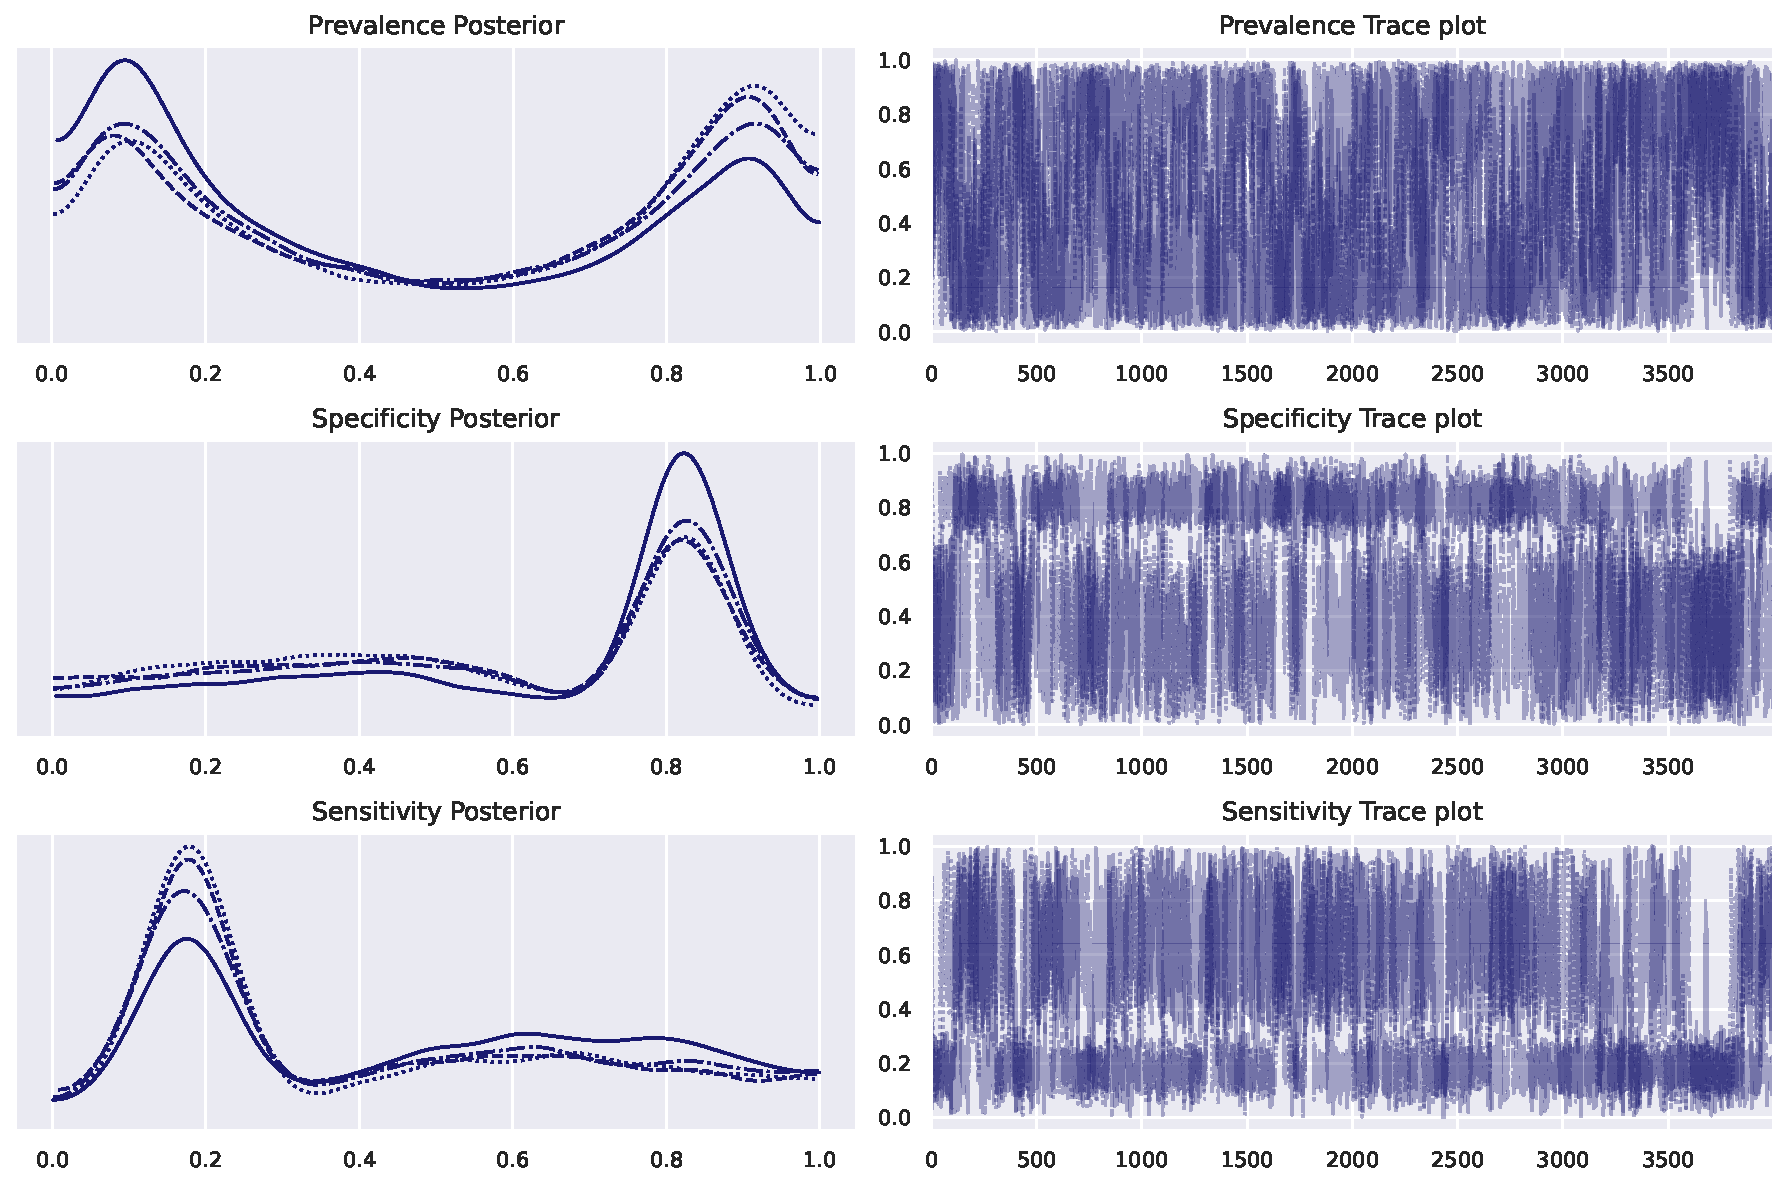
\includegraphics[width=12cm]{posterior-trace-imperfect-tests-identifiability.pdf}
  \fonte{Prepared by the author (2021) with output of Stan.}
\end{figure}

\subsection{Simulated data}

As an initial check for model \eqref{model:imperfect-tests}, we use it to
generate the data to verify if the estimation process is sufficiently
reliable. The experiment is like the one explained in Section
\ref{sec:perfect-test-identifiability}, but with sensitivity and specificity.
We do not recommend vague priors on $\gamma_s$ and $\gamma_e$ because of the
identifiability
problem as mentioned above. We compare the estimates from model
\eqref{model:perfect-tests} in this context. \autoref{table:experiments-imperfect-test} summarizes the
experiments. We use a fixed $\beta = [-0.1, 2.5, 1.4, -1.8, 0.3]$ with
two binary regressors and three continuous drawn from the normal distribution.

\begin{table}[!ht]
  \centering
  \caption{\label{table:experiments-imperfect-test}Experiment settings for the
  simulation of model \eqref{model:imperfect-tests}.}
  \begin{tabular}{ccccc}
  \hline
  Exp & $n$ & $\theta$ & $\gamma_s$ & $\gamma_e$ \\ \hline
  \multicolumn{1}{c}{1} & 100 & 0.1 & 0.9 & 0.8 \\
  \multicolumn{1}{c}{2} & 100 & 0.02 & 0.85 & 0.85 \\
  \multicolumn{1}{c}{3} & 2000 & 0.01 & 0.85 & 0.85 \\
  \multicolumn{1}{c}{4} & 2000 & 0.1 & 0.6 & 0.95 \\
  \multicolumn{1}{c}{5} & 2000 & 0.1 & 0.95 & 0.6 \\ \hline
  \end{tabular}
  \fonte{Prepared by the author (2021). We denote $n$ for number of samples.}
\end{table}

For the first experiment, we placed vague priors on the prevalence and the
effects and informative priors for the sensitivity and specificity. The
algorithm took around 1.87s to perform 4000 iterations  (2000 for a warm-up
and 2000 for sampling). All the basic diagnosis from HMC were good. 
\autoref{fig:trace_plot_experiment1_imperfect_test} summarizes the posterior
distribution. We also applied the first model in this dataset. For this model,
the posterior mean of the prevalence was 0.148 (HDI 94\% 0-0.326), while for
the perfect test model, it was 0.238 (HDI 94\% 0.096-0.375), a biased
estimate. \textcite[p. 1271]{gelman2020bayesian} concludes in its application
that ``uncertainty in the population prevalence is in large part driven by
uncertainty in the specificity.'' However we did not noticed this effect in
this model. \autoref{fig:scatter_plot_posterior_imperfect_tests} presents the
resultant scatter plot of the posterior simulations. Here we observe that all
parameters drive prevalence uncertainty. 

\begin{figure}[ht]
  \centering
  \caption{\label{fig:trace_plot_experiment1_imperfect_test}Posterior distribution
  and trace plot for the first experiment of model
  \eqref{model:imperfect-tests-rds}}
  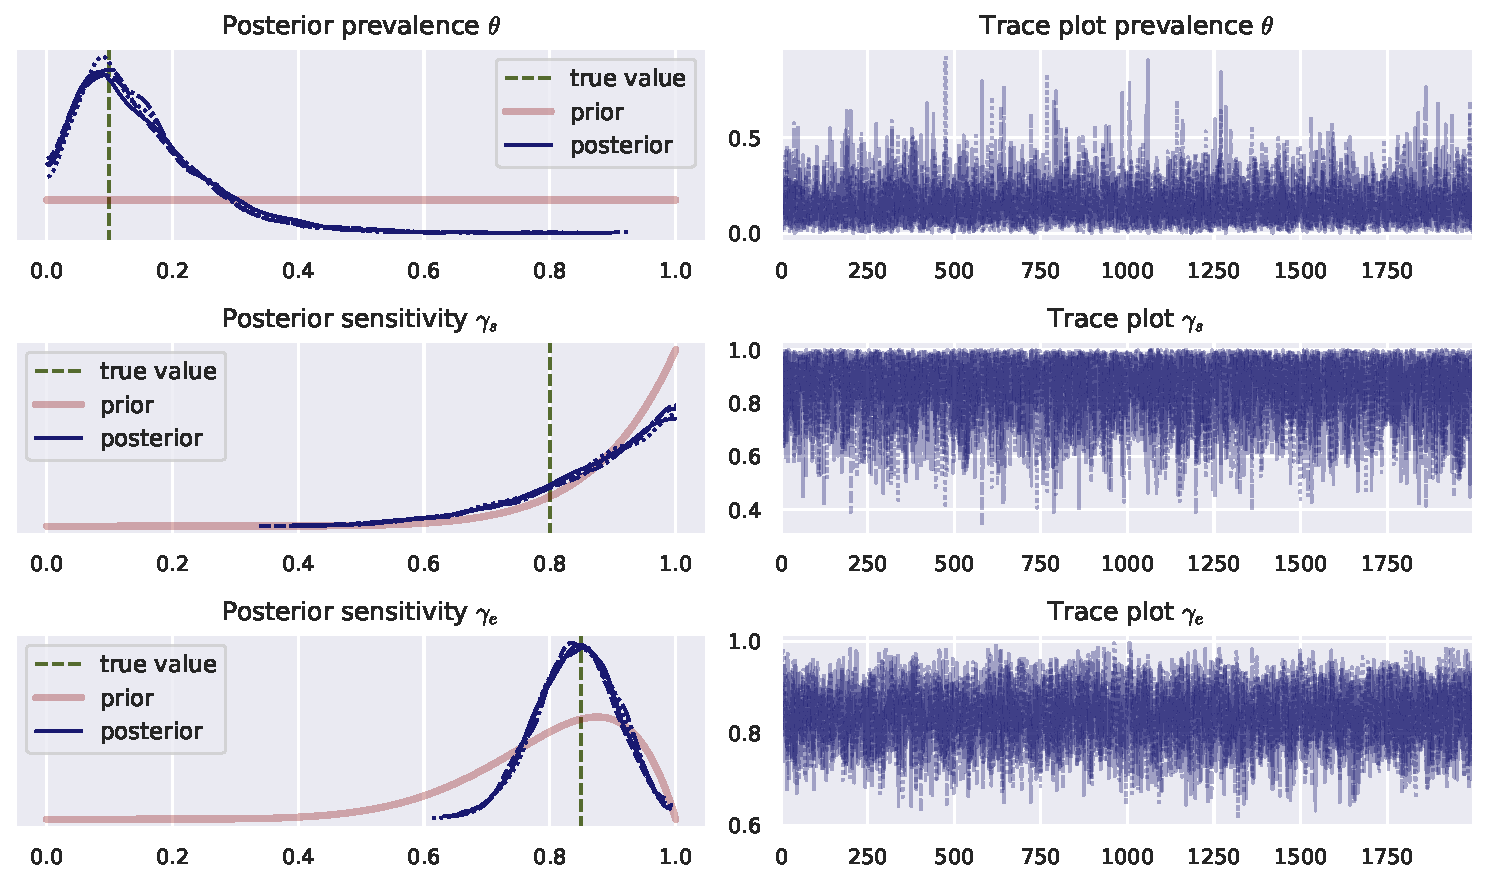
\includegraphics[width=14cm]{trace_plot_experiment1_imperfect_test.pdf}
  \fonte{Prepared by the author (2021) from the Stan sampling result. The
  green line marks the true value for the simulation, while the red line
  represent the density of the prior distribution. Each blue line is a
  posterior distribution sampled from four different chains.}
\end{figure}

\begin{figure}[ht]
  \centering
  \caption{\label{fig:scatter_plot_posterior_imperfect_tests} Scatter plot of
  the posterior simulations of prevalence, specificity, sensitivity and effects of model
  \eqref{model:imperfect-tests-rds}}
  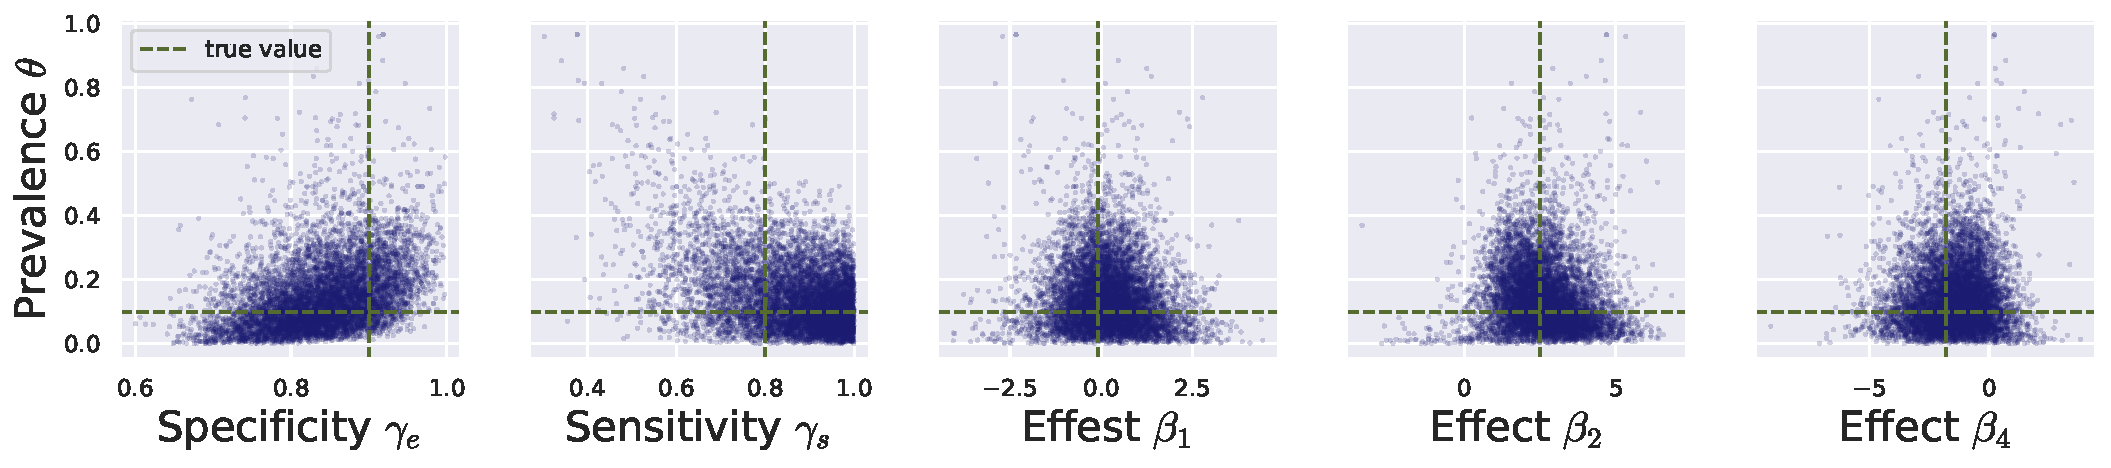
\includegraphics[width=12cm]{scatter_plot_posterior_imperfect_tests.pdf}
  \fonte{Prepared by the author (2021) from the Stan sampling result.}
\end{figure}

To verify frequentist properties, with the same specifications, 
we simulated 1000 datasets varying the test result $Y$ and calculated the 
75\% credible interval. For each experiment, we
verified if the true parameter was included in the corresponding interval.
This happened in 91.5\%, 99.8\%, 83\%, 86.1\%, 72.5\%, 80.1\%, 80.4\%, and 70\% of the
times, respectively for $\theta, \gamma_s, \gamma_e, \beta_1, \dots, \beta_5$.

The second experiment considers the case where the number of samples is not so
high, but prevalece is low. It contrasts with the third experiment where many
more samples are obtained. \autoref{fig:posterior_imperfect_tests_exp2_3}
presents the differences. Notice that the uncertainty was decreased for all
parameters, but specificity decreased the most. Even with a small quantity of
data points, the model had a good performance. When the number of points
increase, 

\begin{figure}[ht]
  \centering
  \caption{\label{fig:posterior_imperfect_tests_exp2_3} Posterior
  distribution for $\theta$, $\gamma_s$ and $\gamma_e$ from model
  \eqref{model:imperfect-tests-rds}}
  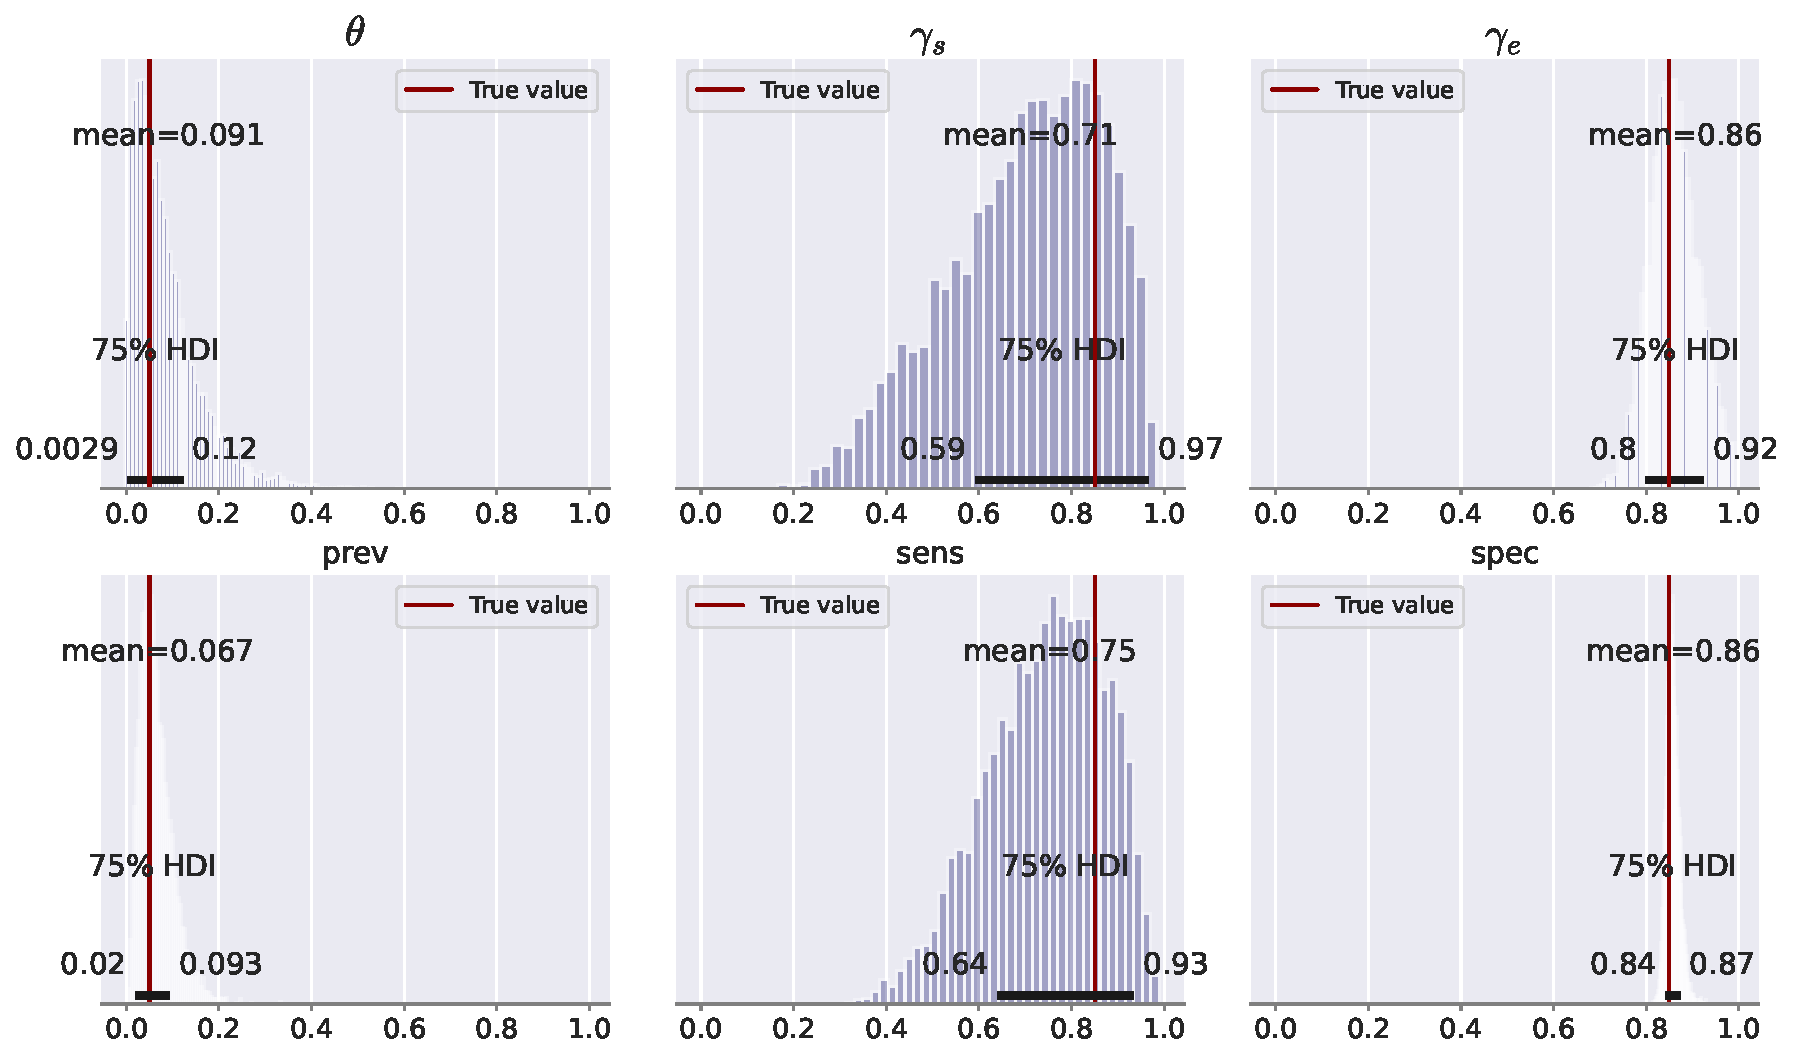
\includegraphics[width=12cm]{posterior_imperfect_tests_exp2_3.pdf}
  \fonte{Prepared by the author (2021) from the Stan sampling result. The red
  line represents the true value for each parameter.}
\end{figure}

\begin{figure}[htbp]
  \centering
  \caption{\label{fig:trace_plot_experiment4_imperfect_test}Posterior distribution
  and trace plot for the fourth experiment of model
  \eqref{model:imperfect-tests-rds}}
  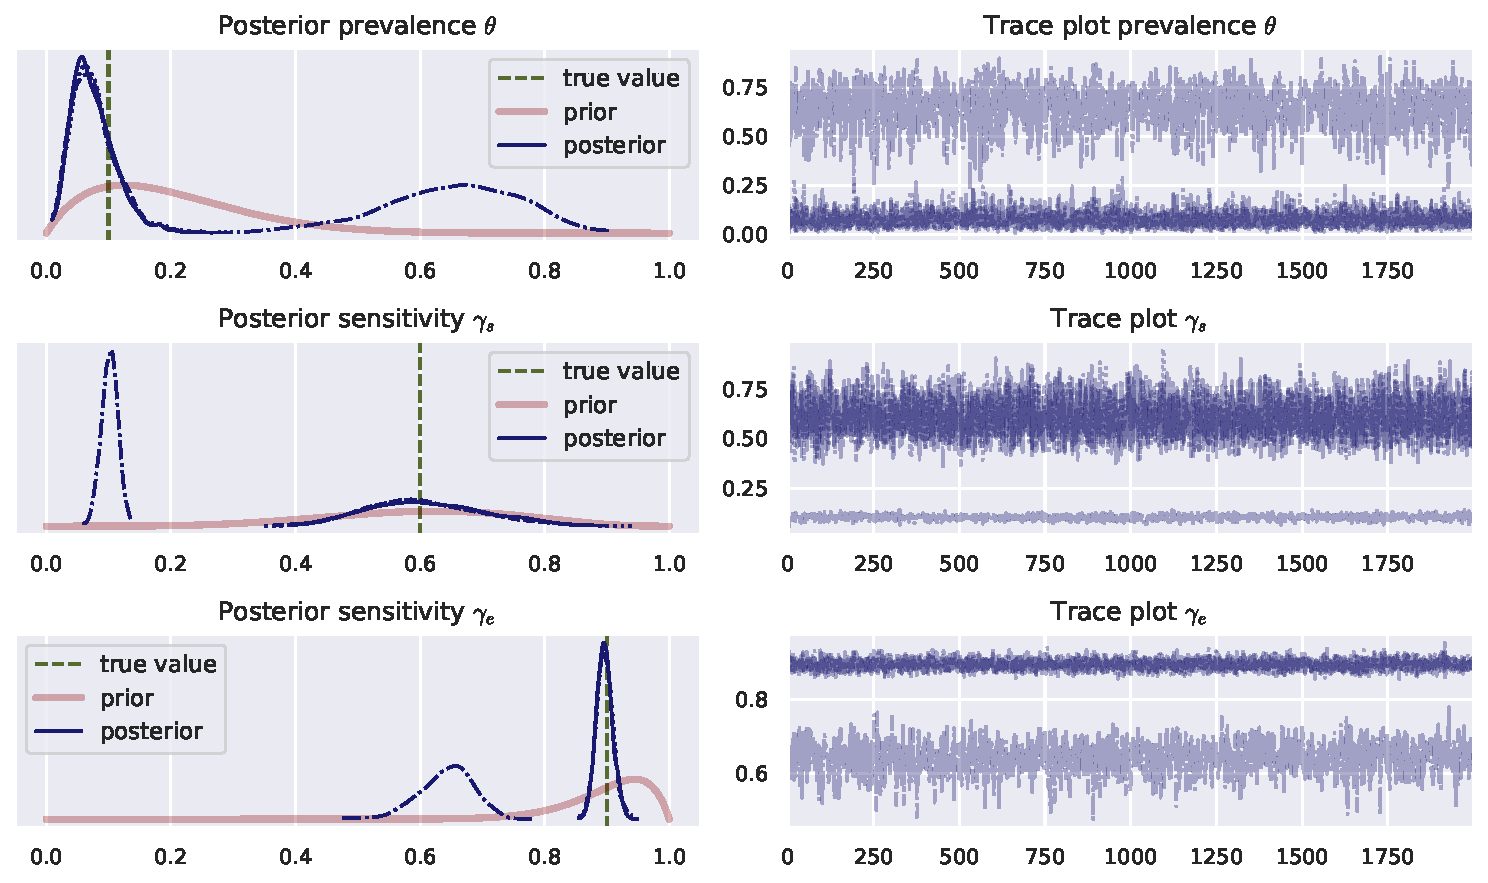
\includegraphics[width=12cm]{trace_plot_experiment4_imperfect_test.pdf}
  \fonte{Prepared by the author (2021) from the Stan sampling result. The
  green line marks the true value for the simulation, while the red line
  represent the density of the prior distribution. Each blue line is a
  posterior distribution sampled from four different chains.}
\end{figure}

The fourth and fifth experiments compare two opposite situations. The former
sets a low sensitivity and a high specificity, while the latter has high
sensitivity and low specificity. These examples are convenient for detecting
the problem with identifiability in high dimensional data. Specifying the hyperparameters with $\alpha_p =
2$,  $\beta_p = 8$, $alpha_s = 6$, $\beta_s = 4$, $\alpha_e = 18$, $\beta_e =
2$, with 2000 iterations for warmup the resulting posterior and trace is given
by \autoref{fig:trace_plot_experiment4_imperfect_test}. Notice that one of the
chains was very far from the tru value driving a very high $\hat{R}$. Although
the result seems awkward, it makes sense under the identifiability problem,
since the chain produces a very similar probability of positive test. A more
strong prior for $\gamma_s$ can handle this effect, which means that the prior
distribution depends on the size of the sample. A similar behavior happens
for the fifth experiment. 

\section{Imperfect tests and respondent-driven sampling}

After understanding the problem when not considering the specificity and the
sensitivity of the diagnostic test for the estimation of $\theta$, we focus on
the sampling strategy studied in Section \ref{sec:respodent_driven_sampling}. 
One problem with RDS is that we
can not make probability statements without making assumptions about the
sampling process. Since the participants recruit their peers, the sampled
individuals depend on the recruiters and whom they recruited. In this section,
we propose a model for the network dependence of RDS extending
\textcite{bastos2012binary}. 

For now, the recruitment graph (see Definition  \ref{def:recruitment-graph}) 
has no uncertainty
incorporated, and we included it as a random effect on the model through a
Conditionally autoregressive (CAR) model (see Section \ref{sec:car-models}) in the Gaussian case.
\textcite{besag1974spatial} introduced
CAR for spatial effects, but they fit in this situation since, by
adjacent sites, we understand recruitment. We remark that for RDS, we
partially observe the corresponding map. If the entire map was available, we
could interpret it as interaction or friendship depending on the population. 

Following the notation of Section \ref{sec:models-rds-process} and Section
\ref{sec:car-models}, we denote $A$ for the adjacency matrix, where $[A]_{ij}
=a_{ij} = 1$ if, and only if, $i$ connects to $j$ and $0$ otherwise; we also
denote $a_{i+} = \sum_j a_{ij}$. Besides the
parameters from model \ref{model:imperfect-tests}, we use $\tau$
for the spatial precision parameter and $\rho$ for controlling the dependence between neighbors. Hence, we specify
the model as follows:
\begin{equation}
  \label{model:imperfect-tests-rds}
  \begin{aligned}
    Y_i \mid p_i &\sim \bern(p_i) \\
    p_i &= \gamma_s\theta_i + (1-\gamma_e)(1 - \theta_i),  \\
    g(\theta_i) &= g(\theta) + \x_i^T\beta + \omega_i,  \\
    \beta  &\sim \N(\mu_{\beta}, \Sigma_{\beta}), \\ 
    \omega_i \mid \omega_j, j \neq i &\sim \N\left(\rho\sum_j a_{ij} \omega_j / a_{i+}, \tau^{-1} / a_{i+}\right), i = 1, \dots, n, 
    \\
    \theta &\sim \betadist(a^p, b^p) \\ 
    \gamma_s &\sim \betadist(a^s, b^s) \\
    \gamma_e &\sim \betadist(a^e, b^e) \\
    \tau &\sim \operatorname{Gamma}(a^{\tau}, b^{\tau}) \\
    \rho & \sim \operatorname{Unif}(0,1/\lambda_{\max}^{-1}).
  \end{aligned}  
\end{equation}
We remind that $\omega \sim \N\left(0, \left[\tau (D - \rho
A)\right]^{-1}\right)$ as discussed in Section \ref{sec:car-models}, such that
$D_{ii} = a_{i+}$. 

The prior specification of $\rho$ has several discussions in the literature.
Since we established that the lower bound is 0, we are saying that there is a
positive correlation between the respondents, which is an usual assumption,
but must be verified for each real application. As we noticed in Section
\ref{sec:car-models}, this correlation is strong only if $\rho$ is close to
$\lambda_{\max}^{-1}$, therefore the uniform distribution contrasts with
this empirical knowledge. \textcite[p. 177]{banerjee2003hierarchical} suggests
the use of beta distribution for $\rho$ with a large mean, ``but this is
controversial since there will typically be little true prior information
available regarding the magnitude of $\alpha$'' \cite[$\alpha$ is the
parameter $\rho$ in our notation.][p.
177]{banerjee2003hierarchical}. \textcite[p. 81]{lee2011comparison} uses a
discrete uniform distribution over $\{0, 0.05, 0.1, \dots, 0.9, 0.95\}$. 

The prior distribution on $\tau$ is also subject to discussion. Since it is a
precision parameter, \textcite[p. 9, Theorem 1]{simpson2017penalising} proves
that if the prior has finite mean, it {\em overfits}, which intuitively means
that the prior puts not enough mass at the base model, in this case the model
without spatial correlation. They calculate a penalized complexity prior for
$\tau$ as the type-2 Gumbel distribution with density 
\begin{equation}
  \label{eq:gumbel-distribution}
  \pi(\tau) = \frac{\lambda}{2}\tau^{-3/2}\exp(-\lambda \tau^{-1/2}), \tau > 0, 
\end{equation}
where $\lambda > 0$ determines the magnitude of the penalty.
\textcite[p. 9]{simpson2017penalising} suggests to specify $U$ and
$\alpha$ so that $\Pr(1 / \sqrt{\tau} > U) = \alpha \implies \lambda =
-\log(\alpha)/U$. This distribution can be rewritten in terms of the standard
deviation $\sigma = 1/ \sqrt{\tau}$ by the Change of Variables
formula as follows
\begin{equation}
  \label{eq:standard-deviation-gumbel}
  \pi(\sigma) = \frac{\lambda}{2}\sigma^{3}\exp(-\lambda \sigma) \cdot 2\sigma^{-3} = \lambda \exp(-\lambda \sigma). 
\end{equation}

\textcite[p. 5]{lee2013carbayes} uses $\sigma^2 \sim \operatorname{Unif}(0,
M_{\sigma})$ with $M_{\sigma} = 1000$ as default based on
\textcite{gelman2006prior} since ``it is difficult to choose the
hyperparameters so that it is non-informative for very small values of''
\cite[p. 4]{lee2013carbayes} referring to specification of a non-informative
inverse-gamma distribution for $\sigma^2$. With that distribution, we
have, by the Change of Variables formula, 
$$
\pi(\tau) = \frac{1}{M_{\sigma}}\tau^{-2}\ind_{\{\tau > 1/M_{\sigma}\}}.
$$

Comparison between parametrization of $\sigma$ and $\tau$ showed that they are
similar in sight of time of execution, energy and divergences, among others
diagnostics. However, the mean estimate of $\sigma$ is more controlled, while 
the median is very similar for both.

\subsection{Identifiability}

This model inherits all the problems with identifiability from the previous
ones. \textcite[p. 3470]{xie2006measures} discusses when two parameters depending on the individual are
summed, one being a CAR component, while the other capturing heterogeneity
among the regions. When $\rho = 1$, the prior on $\omega$ is improper and
property of the posterior must be analysed in each case. Because of that, to
identify the parameter $\theta$, an additional constraint is necessary, such
as 
\begin{equation}
  \label{eq:hard-restriction}
  \sum_{i=1}^n \omega_i = 0.
\end{equation}
Relation \eqref{eq:hard-restriction} is called in optimization as {\em hard
constraint} since the solution must strictly satisfies it. In probability
theory, it would mean to give a point mass distribution for the sum.   
In Stan, a common alternative is to put a {\em soft constraint} such as
\begin{equation}
  \label{eq:soft-restriction}
  \sum_{i=1}^n \omega_i \sim \N(0, 0.0001/n), 
\end{equation}
that serves as a penalty term. 

\subsection{Stan implementation}

Implementing this model was a long process, including several failures and
some successes. This subsection summarizes how the errors happened, how we
detected through diagnoses such as divergences and energy, and how we fixed
them. For the following comparisons, the contact graphs are generated
following an Erdős–Rényi model \cite{erdos2011evolution}, which is the
simplest way to draw a random network. Fixing a number of samples $n$ and a
probability of contact $p$, each node is connected by a link with probability
$p$. The expected number of edges in this graph is $pn(n-1)/2$. To perform a
RDS sampling, we follow \textcite[p. 14670]{baraff2016estimating}: 

\begin{alineas}
  \item 10 seeds are selected at random with probability proportional to their
  degree; 
  \item each participant receives three coupons and has probabilities of 1/3,
  1/6, 1/6 and 1/3 to recruit, respectively, 0, 1, 2 or 3 individuals from their
  contacts;
  \item the last wave of recruitments happens when the number of samples
  is 150. 
\end{alineas}

\subsubsection*{Raw implementation}

The first Stan implementation is exactly as presented in equation
\eqref{model:imperfect-tests-rds}. Coding as we model is an advantage of Stan 
since it improves readability of the code. However this implementation suffers from
some problems concerning the geometry of the parameter space. For this
implementation we treat $\rho$ as a fixed parameter. 1000 iterations of the
algorithm took around 6min. The resulting inferences were not so bad despite
the small number of iterations.
\autoref{fig:energy_plot_inefficient_implementation_stan} presents a
comparative plot between the marginal energy distribution and the distribution
of the transition energy. Since they are very different, it means that the
target distribution has heavy tails, which is challenging for the sampling. In
this case, ``the stochastic exploration between level sets will become so slow that after any finite
number of transitions the exploration of the Markov chain will be
incomplete.'' \cite[p. 44]{betancourt2017conceptual}.

\begin{figure}
  \centering
  \caption{\label{fig:energy_plot_inefficient_implementation_stan}Energy plot
  raw Stan implementation of model \eqref{model:imperfect-tests-rds}}
  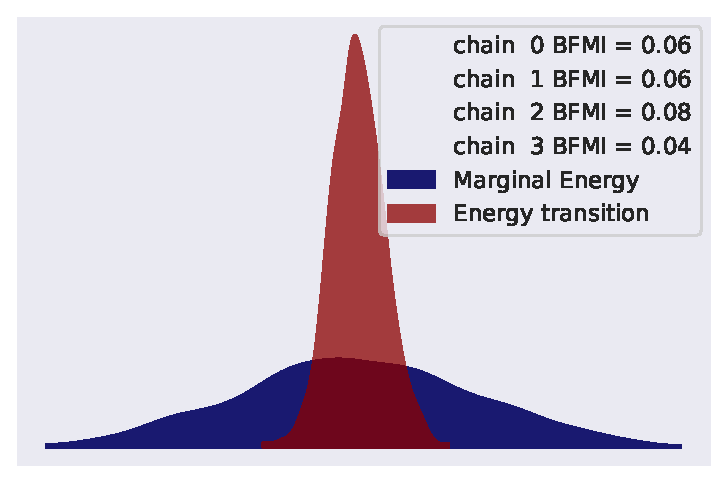
\includegraphics[width=10cm]{energy_plot_inefficient_implementation_stan.pdf}
  \fonte{Prepared by the author (2021) and based on Stan and ArviZ outputs.
  The blue curve is the marginal distribution of the evnergy, while the red 
  is the distribution of the enerrgy transition.}
\end{figure}

\subsubsection*{Vectorization of the variables}

According to the Stan documentation \cite{stan2021vectorization}, the
vectorized form of probability functions and operations such as matrix
products are more efficient than loops and transformed parameters. Because of
that, we apply this suggestion to the implementation. Notice that it does not
solve the problem with the heavy tails of the target distribution, then the
time to make 1000 iterations was around 5min. Although the vectorization did
not prove to be better for the model in particular, we keep on using it given
the general recommendations of the documentation. 

\subsubsection*{Non-centered parameterization}

Parametrization of hierarchical models is a longstanding topic.
\autoref{fig:scatter_plot_inefficient_samples_rds} shows a how the posterior
samples behavior in a hierarchical model. This effect is known as funnel since
there is a high density region with low volume and a low density region with
high volume \cite[p. 1]{betancourt2015hamiltonian}. The posterior correlation
observed can be mitigated through a non-centered parameterization. Taking
$\rho$ fixed, we reparametrize $\omega$ as follows: 
\begin{equation*}
  \begin{split}
    \omega^{\mathrm{raw}}_i &\sim \N(0,1) \\
    \omega &= \tau^{-1/2}V_{\omega} \cdot \omega^{\mathrm{raw}},
  \end{split}
\end{equation*}
where $V_{\omega}V_{\omega}^{*} = (D - \rho A)^{-1}$ is the Cholesky decomposition. We do the
same thing for the effects $\beta$: 
\begin{equation*}
  \begin{split}
    \beta^{\mathrm{raw}}_i &\sim \N(0,1) \\
    \beta &= \mu_{\beta} + V_{\beta} \cdot \beta^{\mathrm{raw}},
  \end{split}
\end{equation*}
where $V_{\beta}V_{\beta}^{*} = \Sigma_{\beta}$. With that little exchange,
the time to run the four chains and 1000 iterations took around 1min, much
better than the previous.
\autoref{fig:energy_plot_non_centered_implementation_stan} shows how this
improves the results on the energy plot. However, this implementation is not
efficient yet, since we are only taking a few iterations. 

\begin{figure}[htb]
  \centering
  \caption{\label{fig:scatter_plot_inefficient_samples_rds}Scatter plot 
  of posterior samples of few parameter from the inefficient Stan implementation of model
  \eqref{model:imperfect-tests-rds} to visualize funnel effects}
  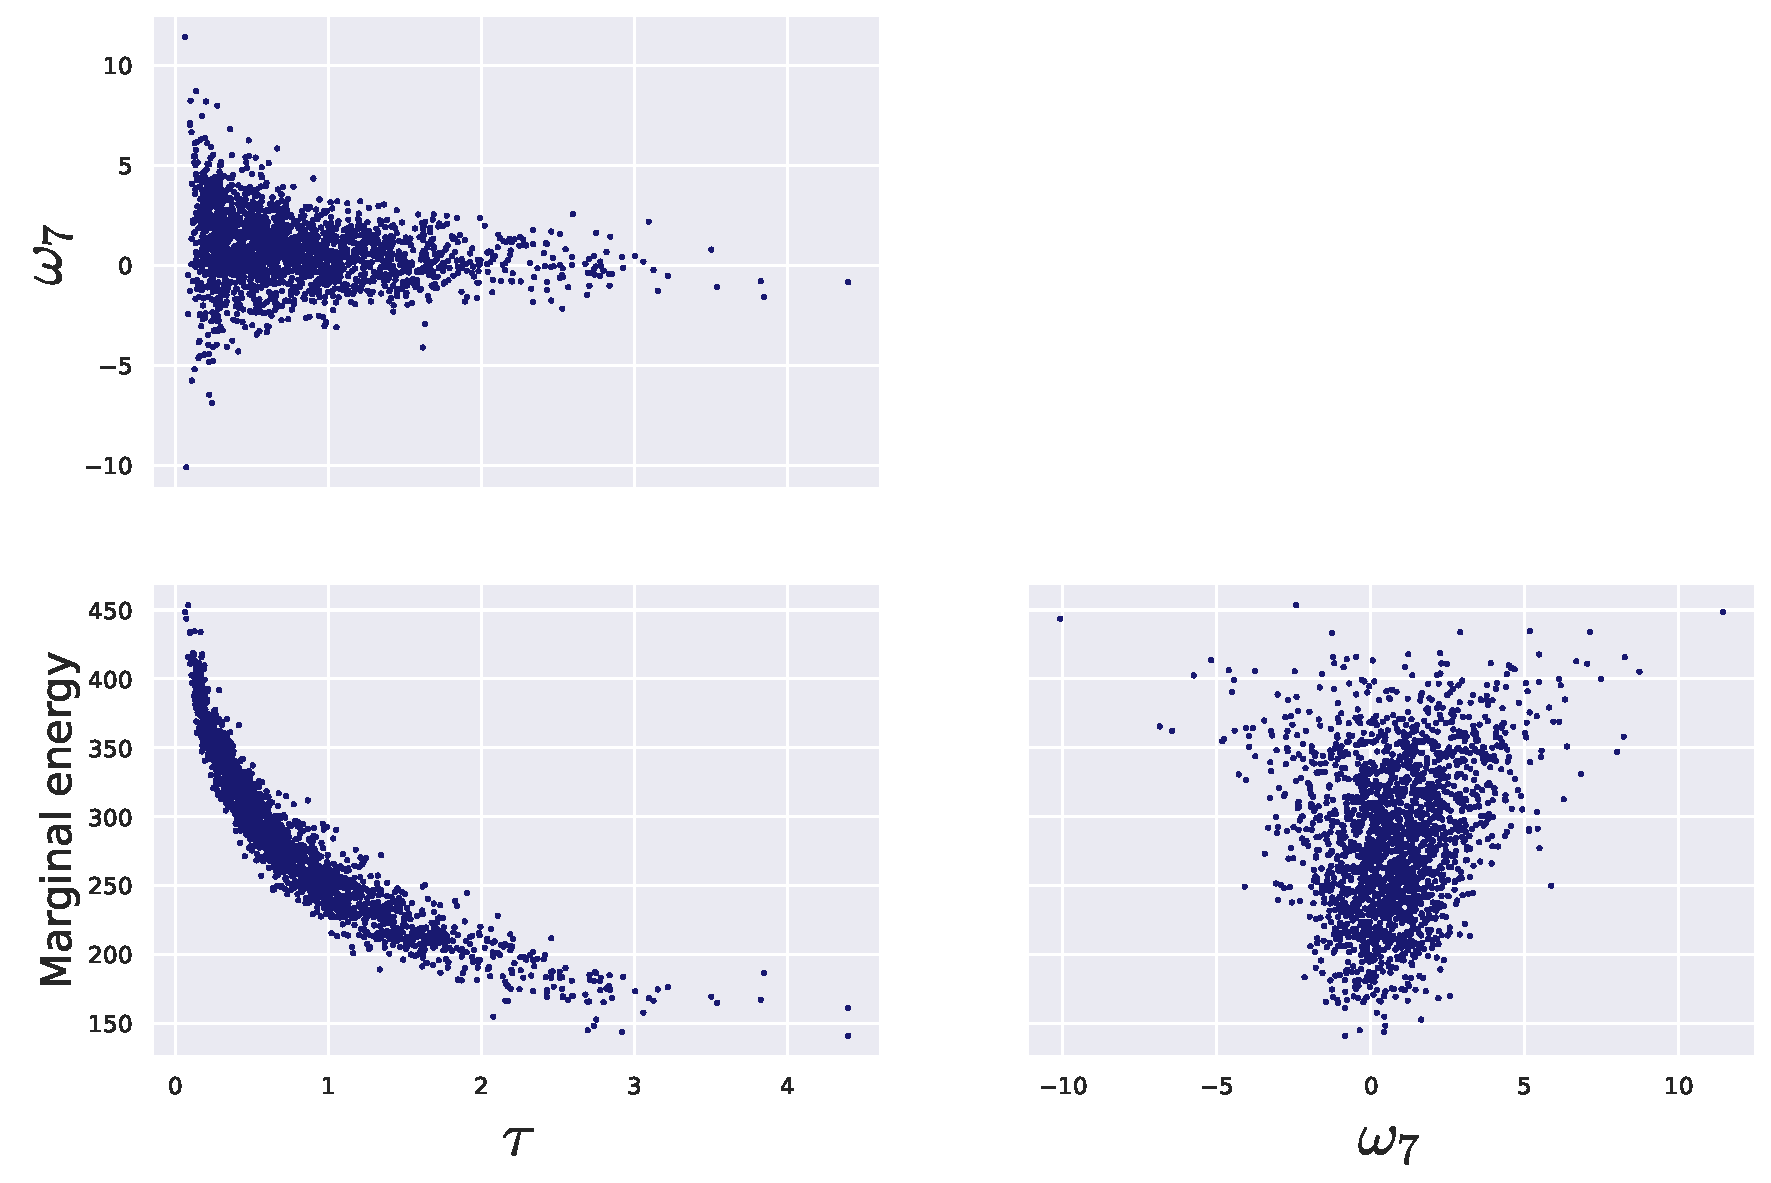
\includegraphics[width=10cm]{scatter_plot_inefficient_samples_rds.pdf}
  \fonte{Prepared by the author (2021) and based on Stan and ArviZ outputs.}
\end{figure}

\begin{figure}[htb]
  \centering
  \caption{\label{fig:energy_plot_non_centered_implementation_stan}Energy plot
  non-centered Stan implementation of model \eqref{model:imperfect-tests-rds}}
  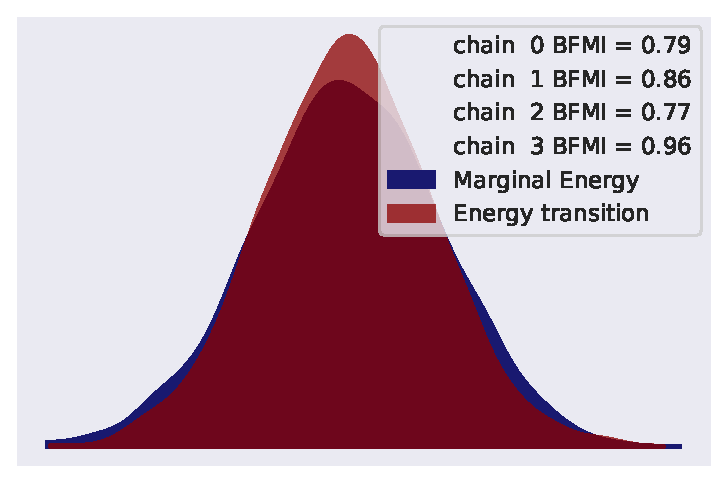
\includegraphics[width=8cm]{energy_plot_non_centered_implementation_stan.pdf}
  \fonte{Prepared by the author (2021) and based on Stan and ArviZ outputs.
  The blue curve is the marginal distribution of the evnergy, while the red 
  is the distribution of the enerrgy transition.}
\end{figure}

\subsubsection*{Efficient implementation}

RDS connection matrix is essentially sparse since the number of edges is at
most four times the number of individuals (one recruiter and three
recruited). Because of that, we follow the efficient implementations of sparse
CAR models
from \textcite{donegan2021spatial} and \textcite{exactcar}. The probability
density of a multivariate normal distribution with zero mean is 
\begin{equation}
  \label{eq:multivariate_normal}
  f_{\omega}(\omega \mid \tau, \rho) = \frac{1}{\sqrt{(2\pi)^n\det(\Sigma^{-1})}
  }\exp\{-\frac{1}{2}\omega^T\Sigma^{-1}\omega\}, 
\end{equation}
where $\Sigma^{-1} = \tau(D - \rho A)$. \textcite[p. 955]{jin2005generalized}
proves the following relation
$$
\det(\tau(D - \rho A)) = \tau^n \det(D - \rho A) \propto \tau^n \prod_{i=1}^n (1 - \rho \lambda_i), 
$$
where $\lambda_1, \dots, \lambda_n$ are the eigenvalues of $D^{-1/2} A
D^{-1/2}$. Notice that $\{\lambda_i\}_{i=1}^n$ are calculated before of the
HMC algorithm. We also have that $\omega^T(D - \rho A)\omega = \omega^T D \omega - \rho \omega^T A
\omega$. Since $D$ is a diagonal matrix, $\omega^T D \omega = \sum_{i=1}^n
D_ii\omega_i^2$ which can be easily calculated. Moreover, by the sparsity of $A$,
$\omega^T A \omega$ can be performed with sparse matrix operations. 

Given that Stan receives the log density and constants are not necessary,
\eqref{eq:multivariate_normal} can be simplified to 
\begin{equation*}
  \log f_{\omega}(\omega \mid \tau, \rho) = \frac{n}{2}\log(\tau) + 
  \frac{1}{2}\sum_{i=1}^n(1 - \rho \lambda_i) - \frac{\tau}{2}\omega^T(D - \rho A)\omega.
\end{equation*}

The time to perform 1000 iterations was around 8s, which is a pretty good
reduction compared to the previous implementations. Despite that, the
efficient implementation has the disadvantage of not
allowing to rescale the multivariate normal distribution, given that matrix $V_{\omega}$ does not have
a sparse representation. Therefore, the energy plot is very similar to
\autoref{fig:energy_plot_inefficient_implementation_stan}. The scatter plot is
aso very similar to \autoref{fig:scatter_plot_inefficient_samples_rds}, but
since the we can draw more samples without worrying about time of execution,
the funnel effects is more evident as presented in \autoref{fig:scatter_plot_efficient_samples_rds}.

\begin{figure}[htb]
  \centering
  \caption{\label{fig:scatter_plot_efficient_samples_rds}Scatter plot 
  of posterior samples of few parameter from the efficient Stan implementation of model
  \eqref{model:imperfect-tests-rds} to visualize funnel effects}
  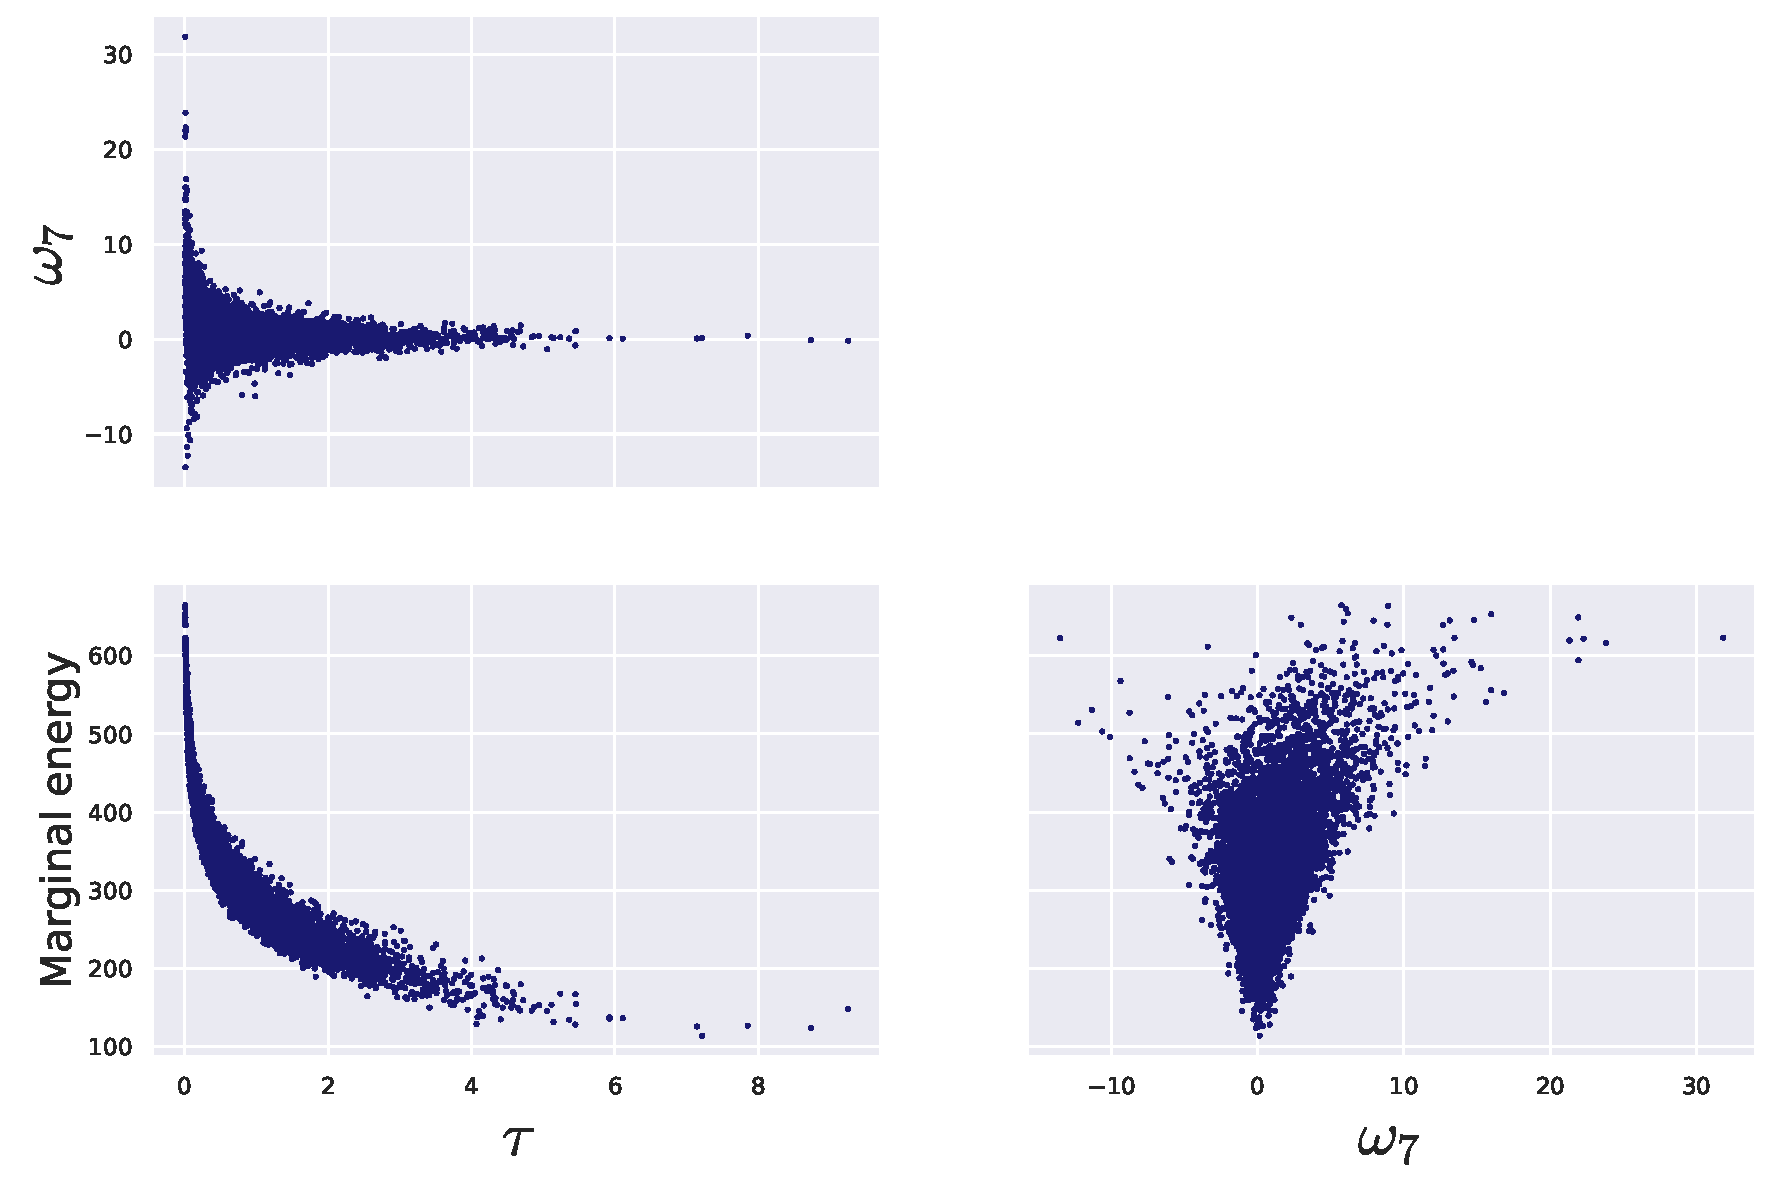
\includegraphics[width=10cm]{scatter_plot_efficient_samples_rds.pdf}
  \fonte{Prepared by the author (2021) and based on Stan and ArviZ outputs.}
\end{figure}

Although the Cholesky decomposition of $D - \rho A$ is not sparse, we can
rescale the parameter $\tau$ from the sparse re\begin{equation*}
  \log f_{\omega}(\omega \mid \tau, \rho) = \frac{n}{2}\log(\tau) + 
  \frac{1}{2}\sum_{i=1}^n(1 - \rho \lambda_i) - \frac{\tau}{2}\omega^T(D - \rho A)\omega.
\end{equation*}presentation of CAR model. Let 
\begin{align*}
  \omega^{\mathrm{scaled}}_i &\sim \N(0,1) \\ 
  \omega &= 1/\sqrt{\tau} \cdot \omega^{\mathrm{scaled}}.
\end{align*}

The efficient representation of the density of $\omega^{\mathrm{sacaled}}$ is 
\begin{equation*}
  \log f_{\omega}(\omega \mid \rho) = \frac{1}{2}\sum_{i=1}^n(1 - \rho \lambda_i) - \frac{1}{2}\omega^T(D - \rho A)\omega,
\end{equation*}
which is equivalent to $\log f_{\omega}(\omega \mid \tau=1, \rho)$. 

\subsubsection*{Scaling the precision in the efficient implementation}

\subsection{Simulated data}

\begin{alineas}
  \item More sparse matrices (RDS data is very sparse) is generating the funil
  we do not want to see. This is not connected to the number of connected
  components. In order to see that, a simple example with the Erdos-Renyi
  Random Graph can answer to us. In the sparse case, the number of edges is
  $O(n)$ with $p=1/n$. If $p=1$, the number of edges is $O(n^2)$ and the funil
  disappears. This problem does not appear in the poisson model. 
\end{alineas}

\subsection{Including uncertainty about the recruitment graph}


% RDS has the constraint of being without replacement. For that reason, we do
% not observe all links among the samples \cite[]{crawford2016}. Considering the
% model developed by Crawford, we can model the
% matrix $Q$ as {\em Exponential Random Graph Model} (ERGM). Define the
% following 

% \begin{alineas}
%   \item $\boldsymbol{s} = \tril(QC)^T \boldsymbol{1} + C^Tu$, such that $Q$ is the
%   adjacency matrix of the recruited subjects, $C$ is the {\em Coupon Matrix},
%   $u$ the vector of the number of edge ends belonging to each vertex
%   (in the order of recruitment) that are not connected to any other sampled
%   vertex, and $\tril(M)$ the lower triangle of $M$. 

%   \item $T(Q) = -\lambda \boldsymbol{s}$, such that $\lambda$ is the rate of
%   the recruitment time. 

%   \item $V(Q) = \sum_{k \text{ is not seed}} \log(\lambda \boldsymbol{s}_k)$
  
%   \item $w = (0, t_2 - t_1, ..., t_n - t_{n-1})$ is the worst.
%   3. Comparison between parametrization of sigma and tau showed that they are
%   similar in sight of time of execution, energy and divergences, among others
%   diagnostics. However, the mean estimate of sigma is more controlled. The
%   median estimate is very similar. This happens because there are a few very
%    vector of the waiting times between
%   recruitments.  
% \end{alineas}

% Therefore $\Pr(Q|w) \propto \exp[T(Q)^Tw + V(Q)]$. With that, the model
% becomes 

% \begin{equation}
%   \begin{aligned}
%     T_i &\sim \bern(p_i) \\
%     p_i &= \gamma_s\theta_i + (1-\gamma_e)(1 - \theta_i),  \\
%     g(\theta_i) &= g(\theta) + \x_i^T\beta + \omega_i,  \\
%     \omega_i|\{\omega_j\}_{j\neq i}, \tau &\sim \N\left(\rho\sum_j q_{ij}\omega_j/q_{i+}, \tau^2/q_{i+}\right) \\
%     Q|w &\propto \exp[T(Q)^Tw + V(Q)] \\
%     \lambda &\sim \Gamma(a^{\lambda}, b^{\lambda}), \\ 
%     \beta &\sim \N(\mu, \Sigma), \\ 
%     \theta &\sim \betadist(a^p, b^p) \\
%     \gamma_s &\sim \betadist(a^s, b^s), \\
%     \gamma_e &\sim \betadist(a^e, b^e), \\  
%     \tau &\sim \N^+(0,\sigma^2_{\tau}).
%   \end{aligned}  
% \end{equation}
% The problem with this model is that we are assigning a posterior distribution
% for $Q$.

\section{Model extensions}

Several characteristics of RDS were not include in the previous model, such as
homophily, bottlenecks, and sampling weights. This section aims to build some
options for these aspects and establish future works in that line. 

\begin{alineas}
  \item {\em Homophily model}: \cite{yauck2021general} 
  \item {\em Sampling weights}: GLM weighted
  \item {\em Bottlenecks}
\end{alineas}

\section{Mispecified data simulation}

